\begin{figure}[!ht]
  \centering
  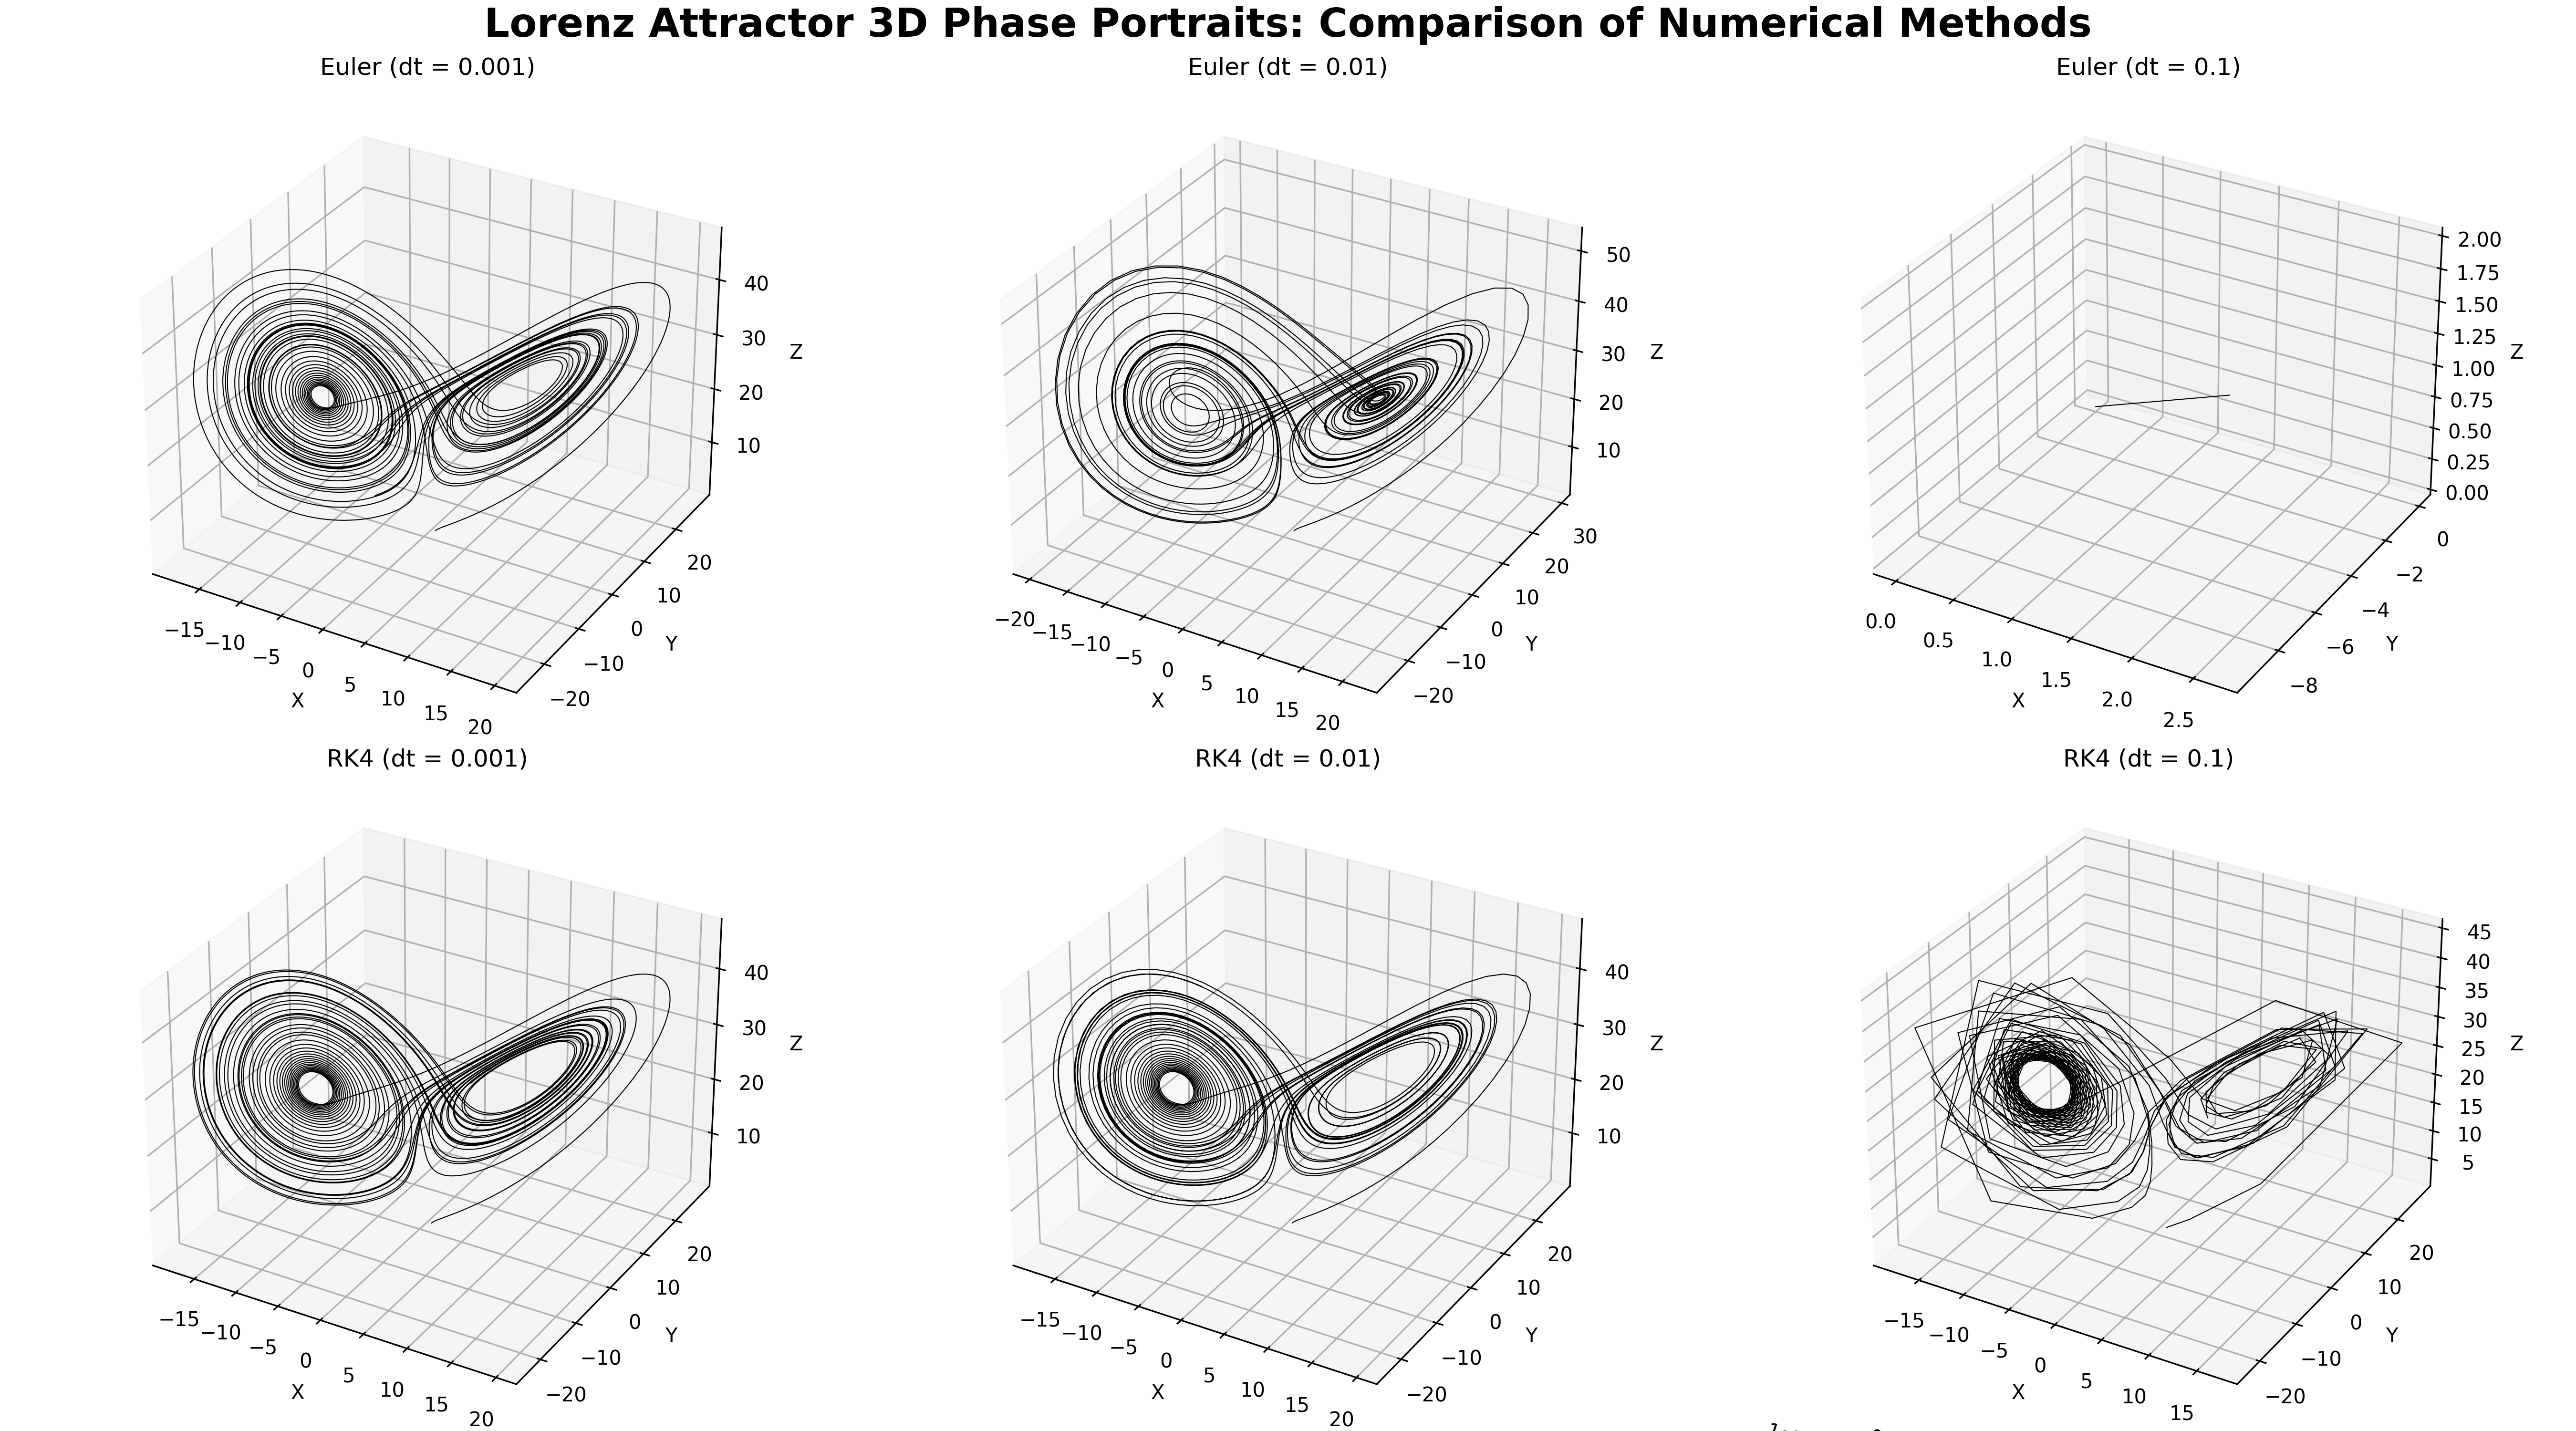
\includegraphics[width=1.0\linewidth]{images/phase_portraits1.1.4.png} 
  \caption{Lorenz attractor with initial state (1.0,1.0,1.0) and time step (0.001, 0.01, 0.1), and total simulation time of 40 seconds,  For $\Delta t > 0.01$, the solution is not stable enough to reliably reproduce the attractor shape\cite{youngaryanLorenzPlot1.1.4_image}}
  \label{fig:lorenz_vis}
\end{figure}


\begin{figure}[!ht]
  \centering
  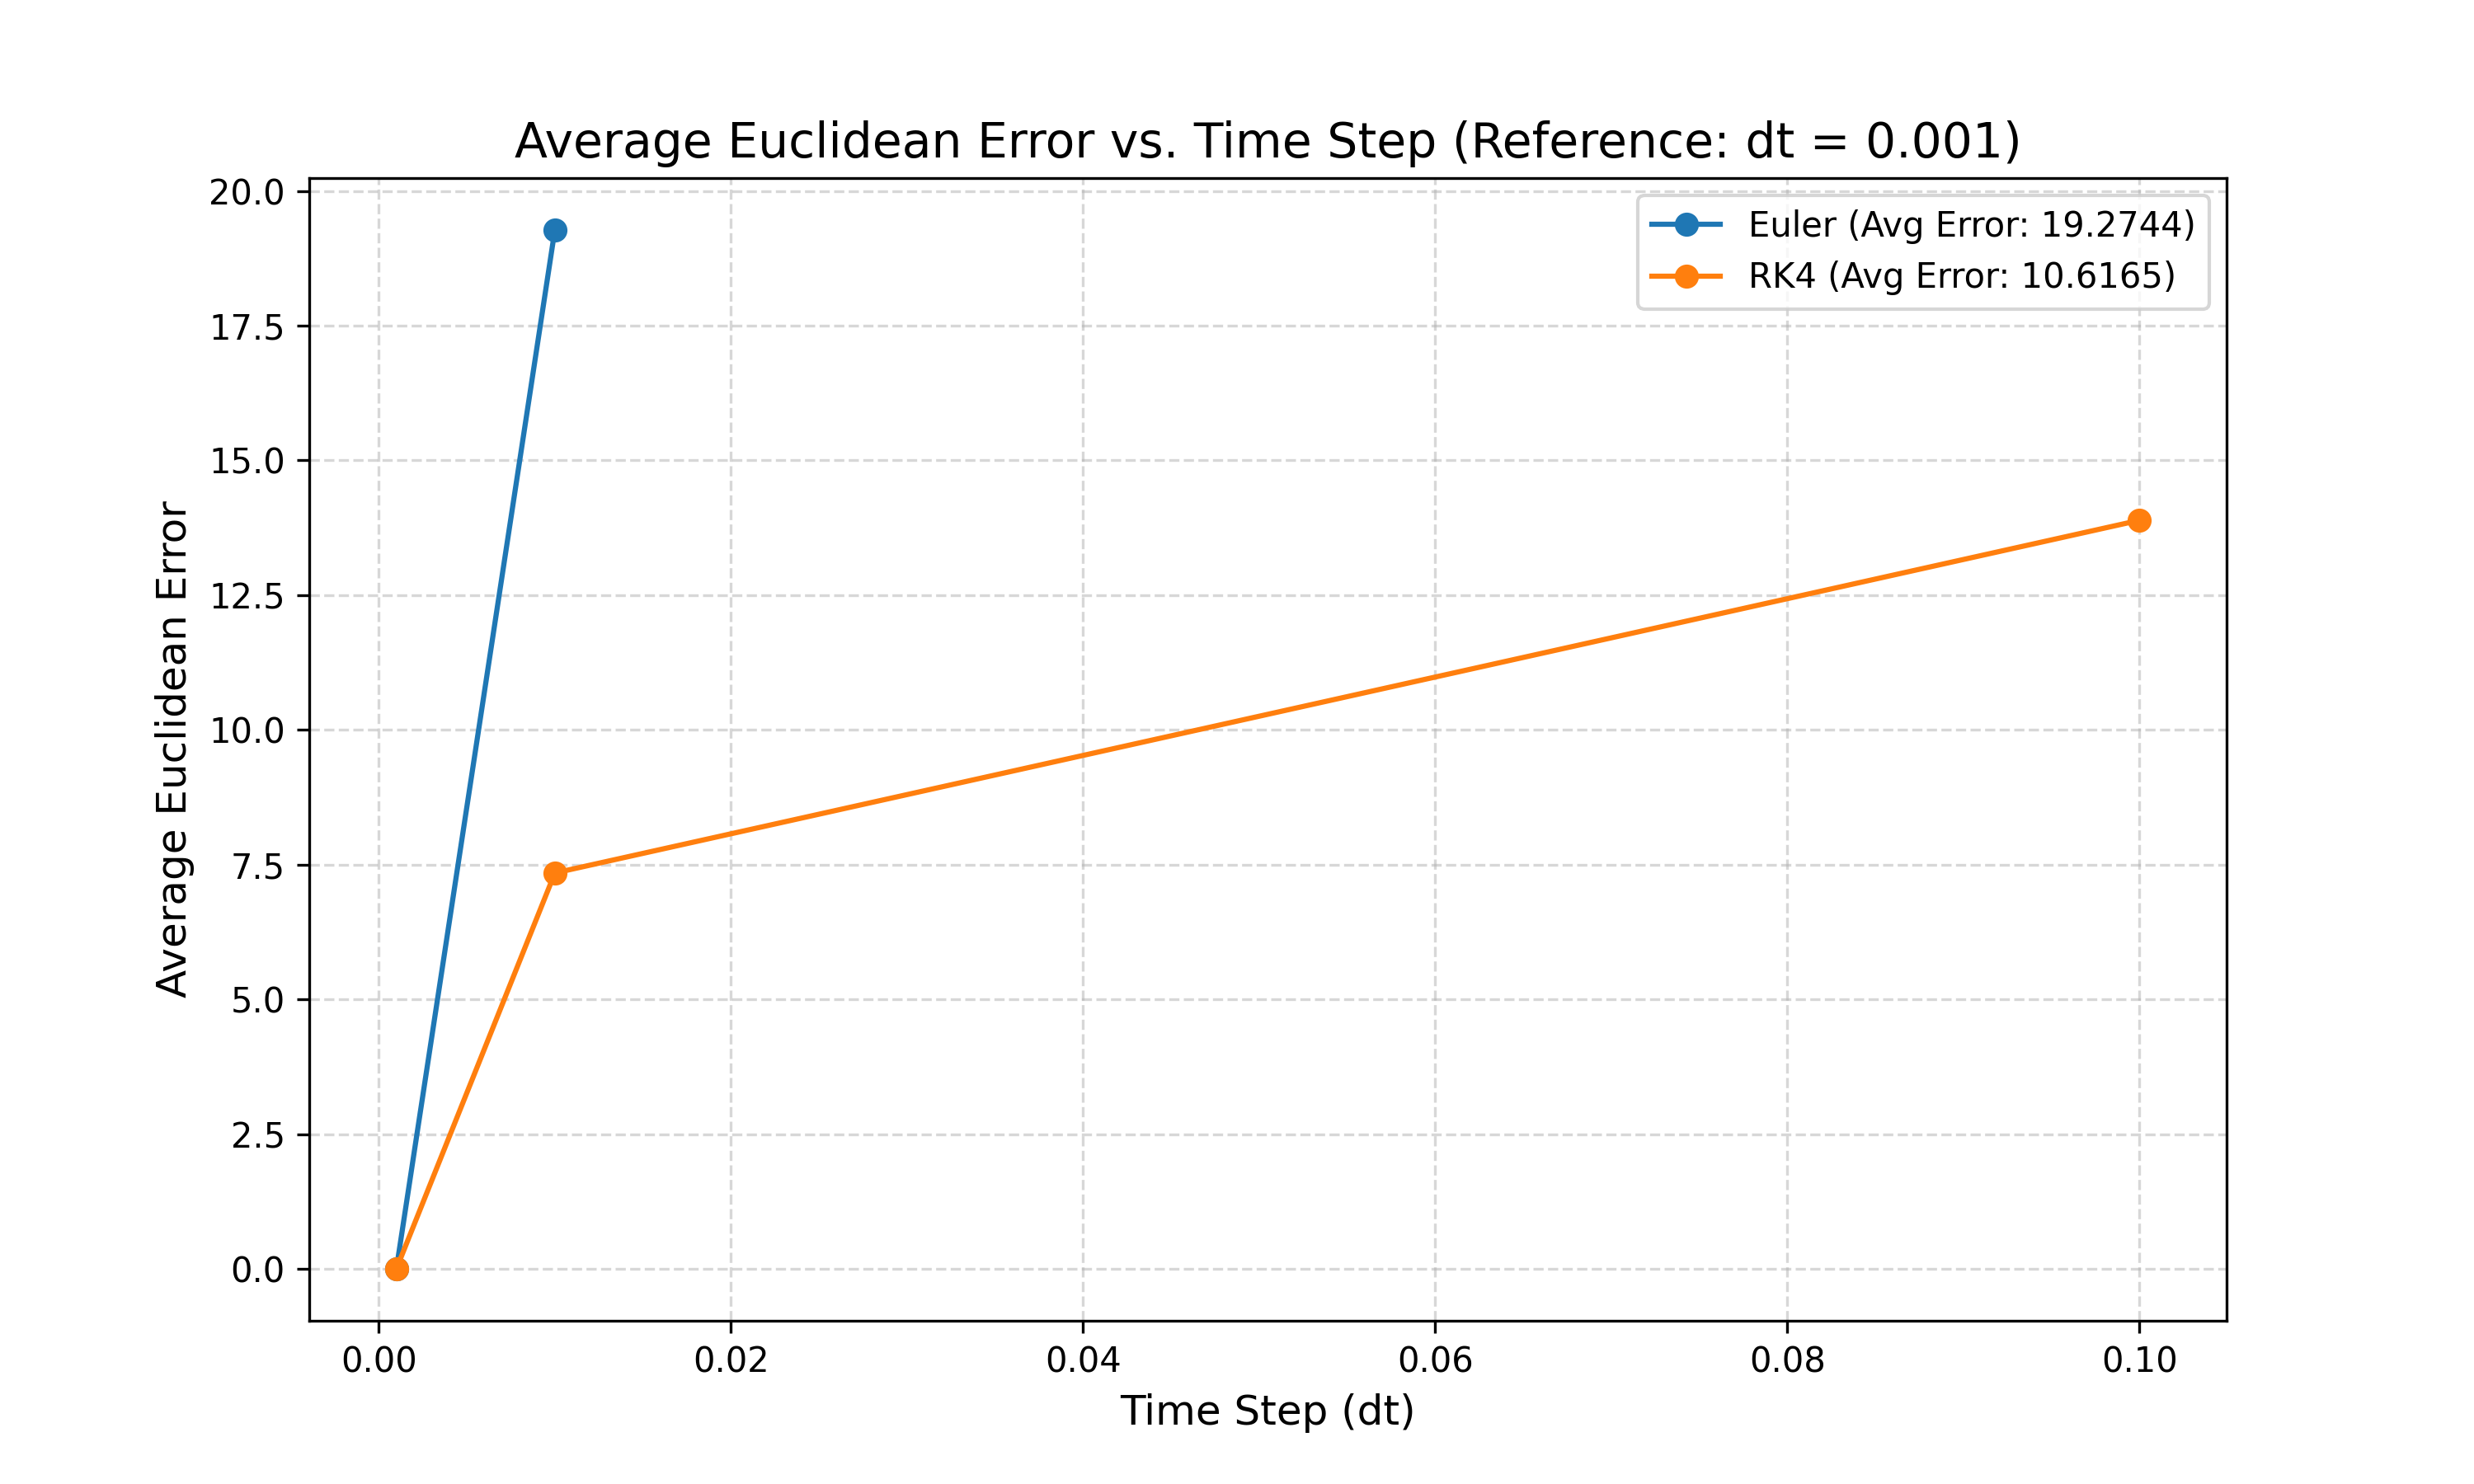
\includegraphics[width=1.0\linewidth]{images/error_comparison1.1.4.png} 
  \caption{Lorenz attractor error analysis with initial state (1.0,1.0,1.0) and time step (0.001, 0.01, 0.1), and total simulation time of 40 seconds,  For $\Delta t > 0.01$, the solution is not stable enough to reliably reproduce the attractor shape\cite{youngaryanLorenzPlot1.1.4_image}}
  \label{fig:error_comparison1.1.4}
\end{figure}

\begin{figure}[!ht]
  \centering
  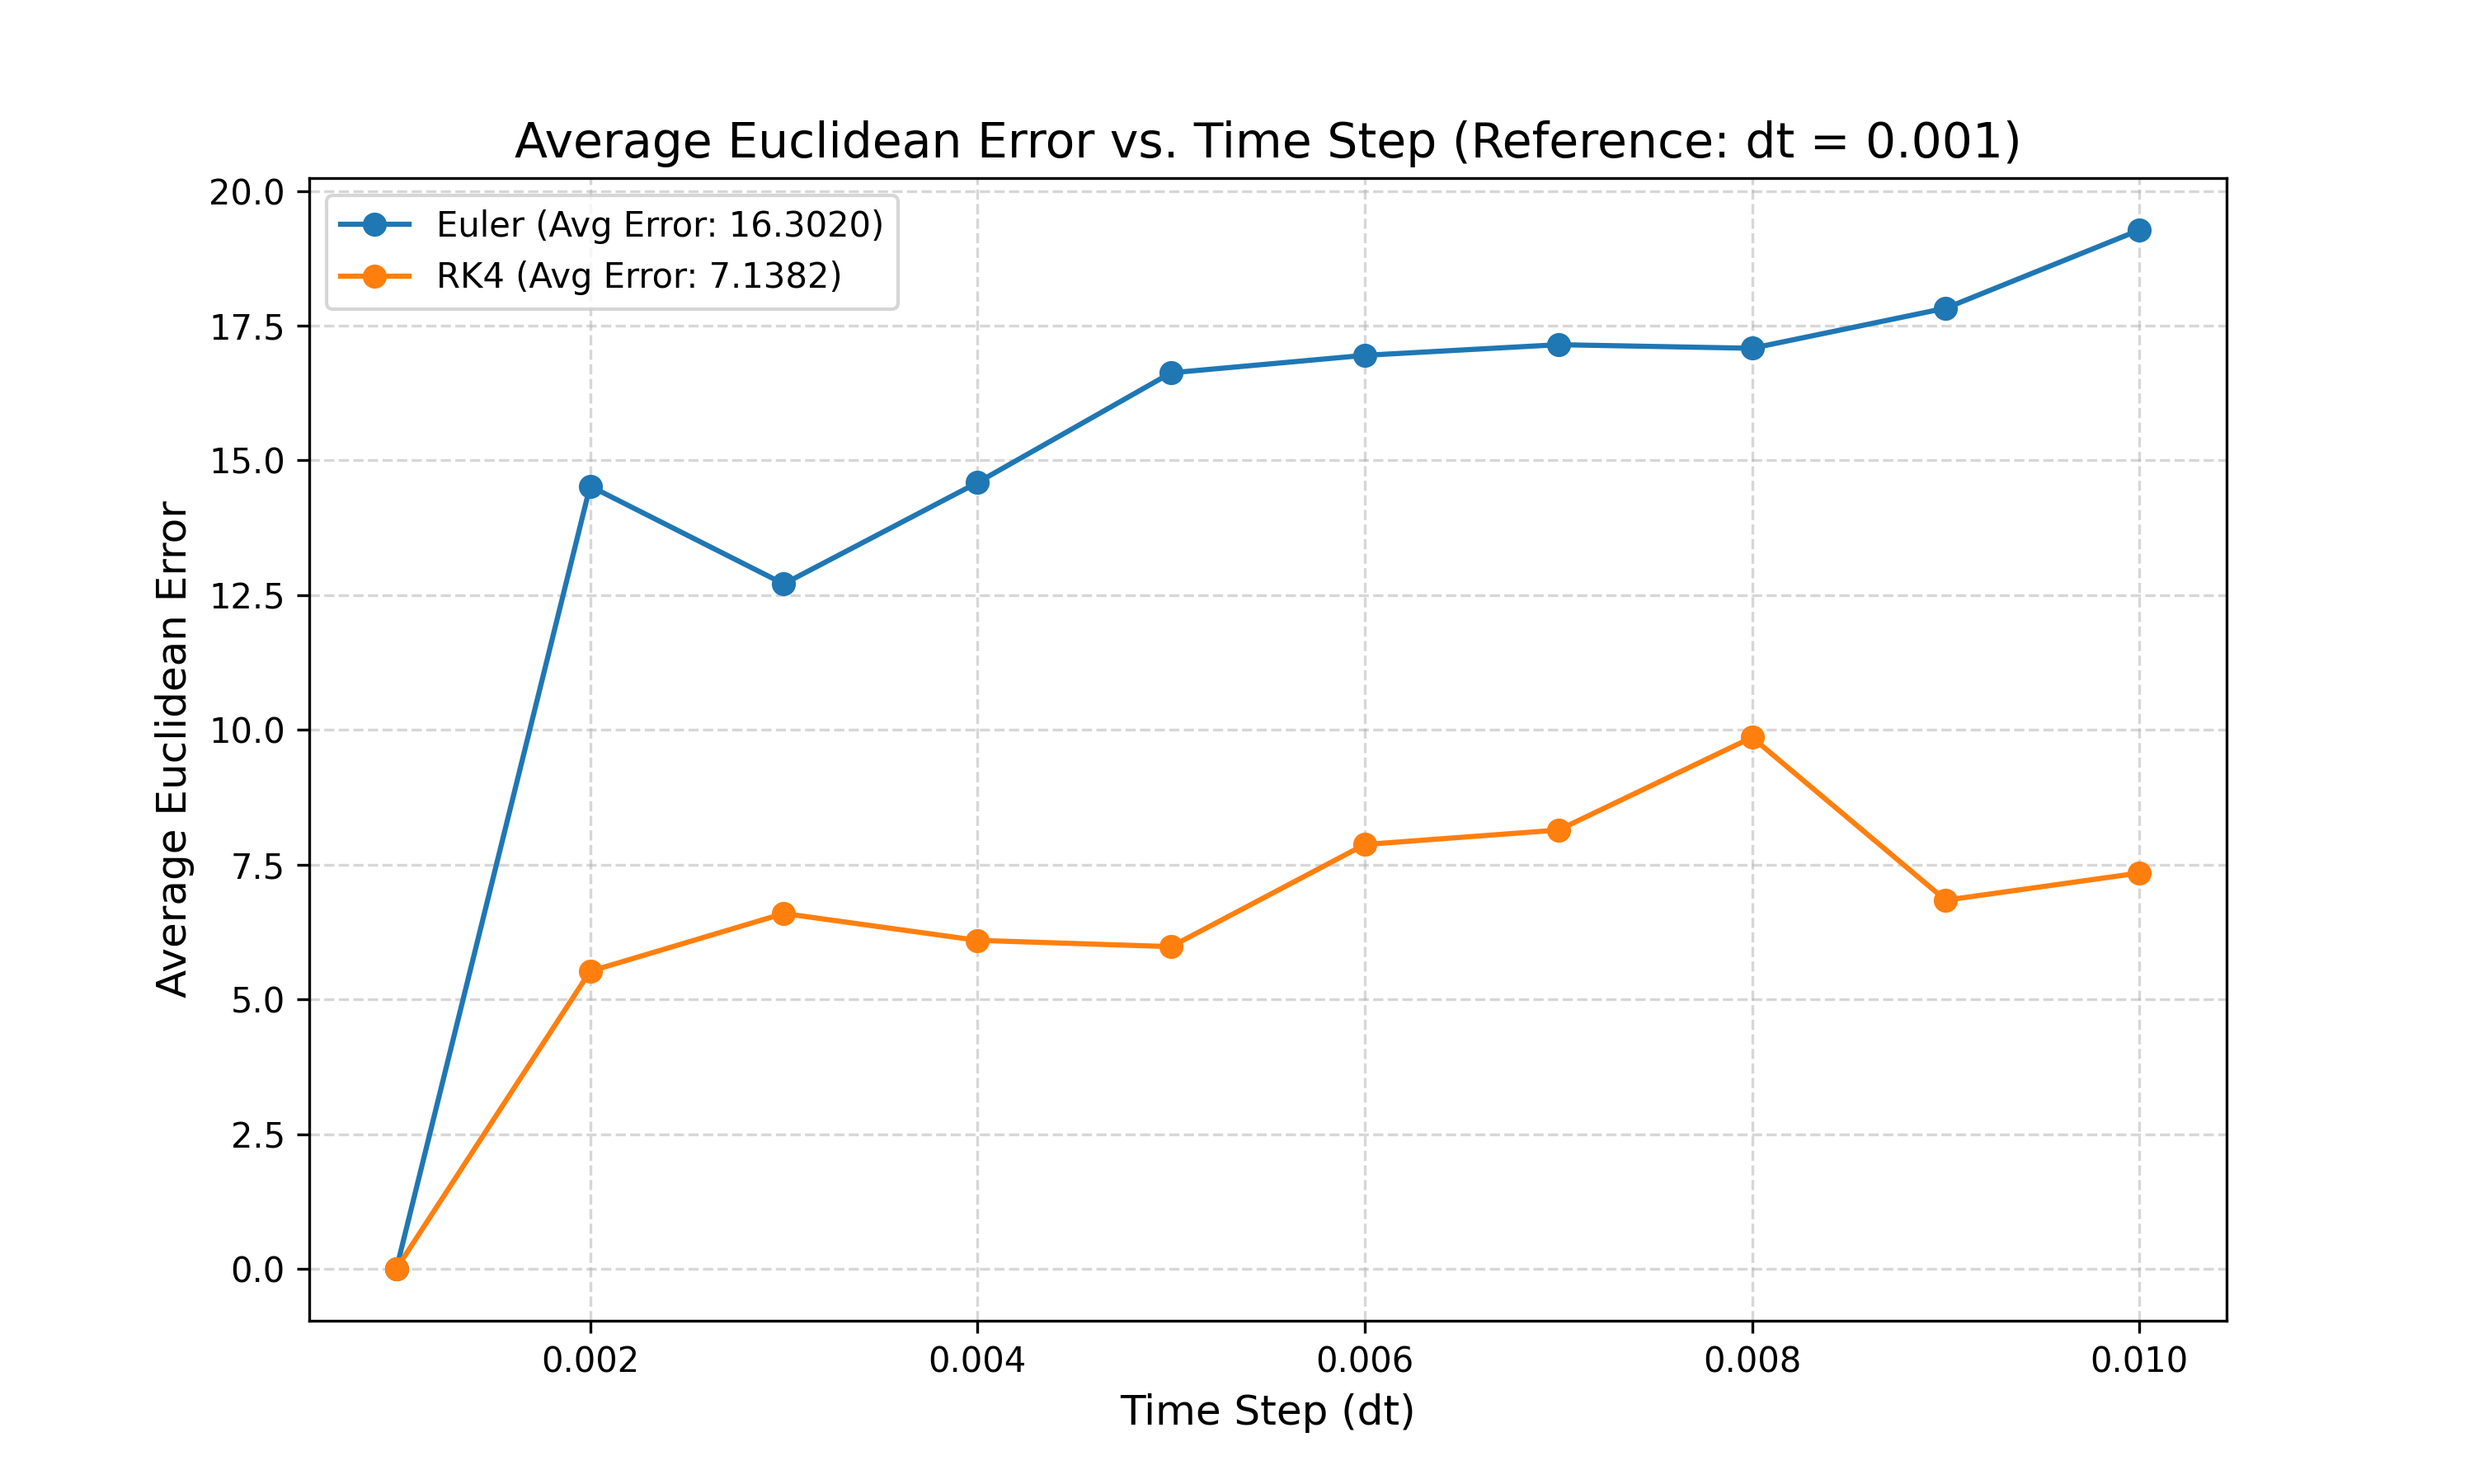
\includegraphics[width=0.9\linewidth]{images/error_comparison_same_times.png}
  \caption{Lorenz attractor error analysis with initial state \((1.0, 1.0, 1.0)\), 1000 different time steps between \((0.0001 and 0.001)\), and a total simulation time of 40 seconds. this experiment is to compare the mean error of the two methods\cite{youngaryanLorenzError1.1.4_image}.}
  \label{fig:error_comparison_same_times}
\end{figure}





\begin{figure}[!ht]
  \centering
  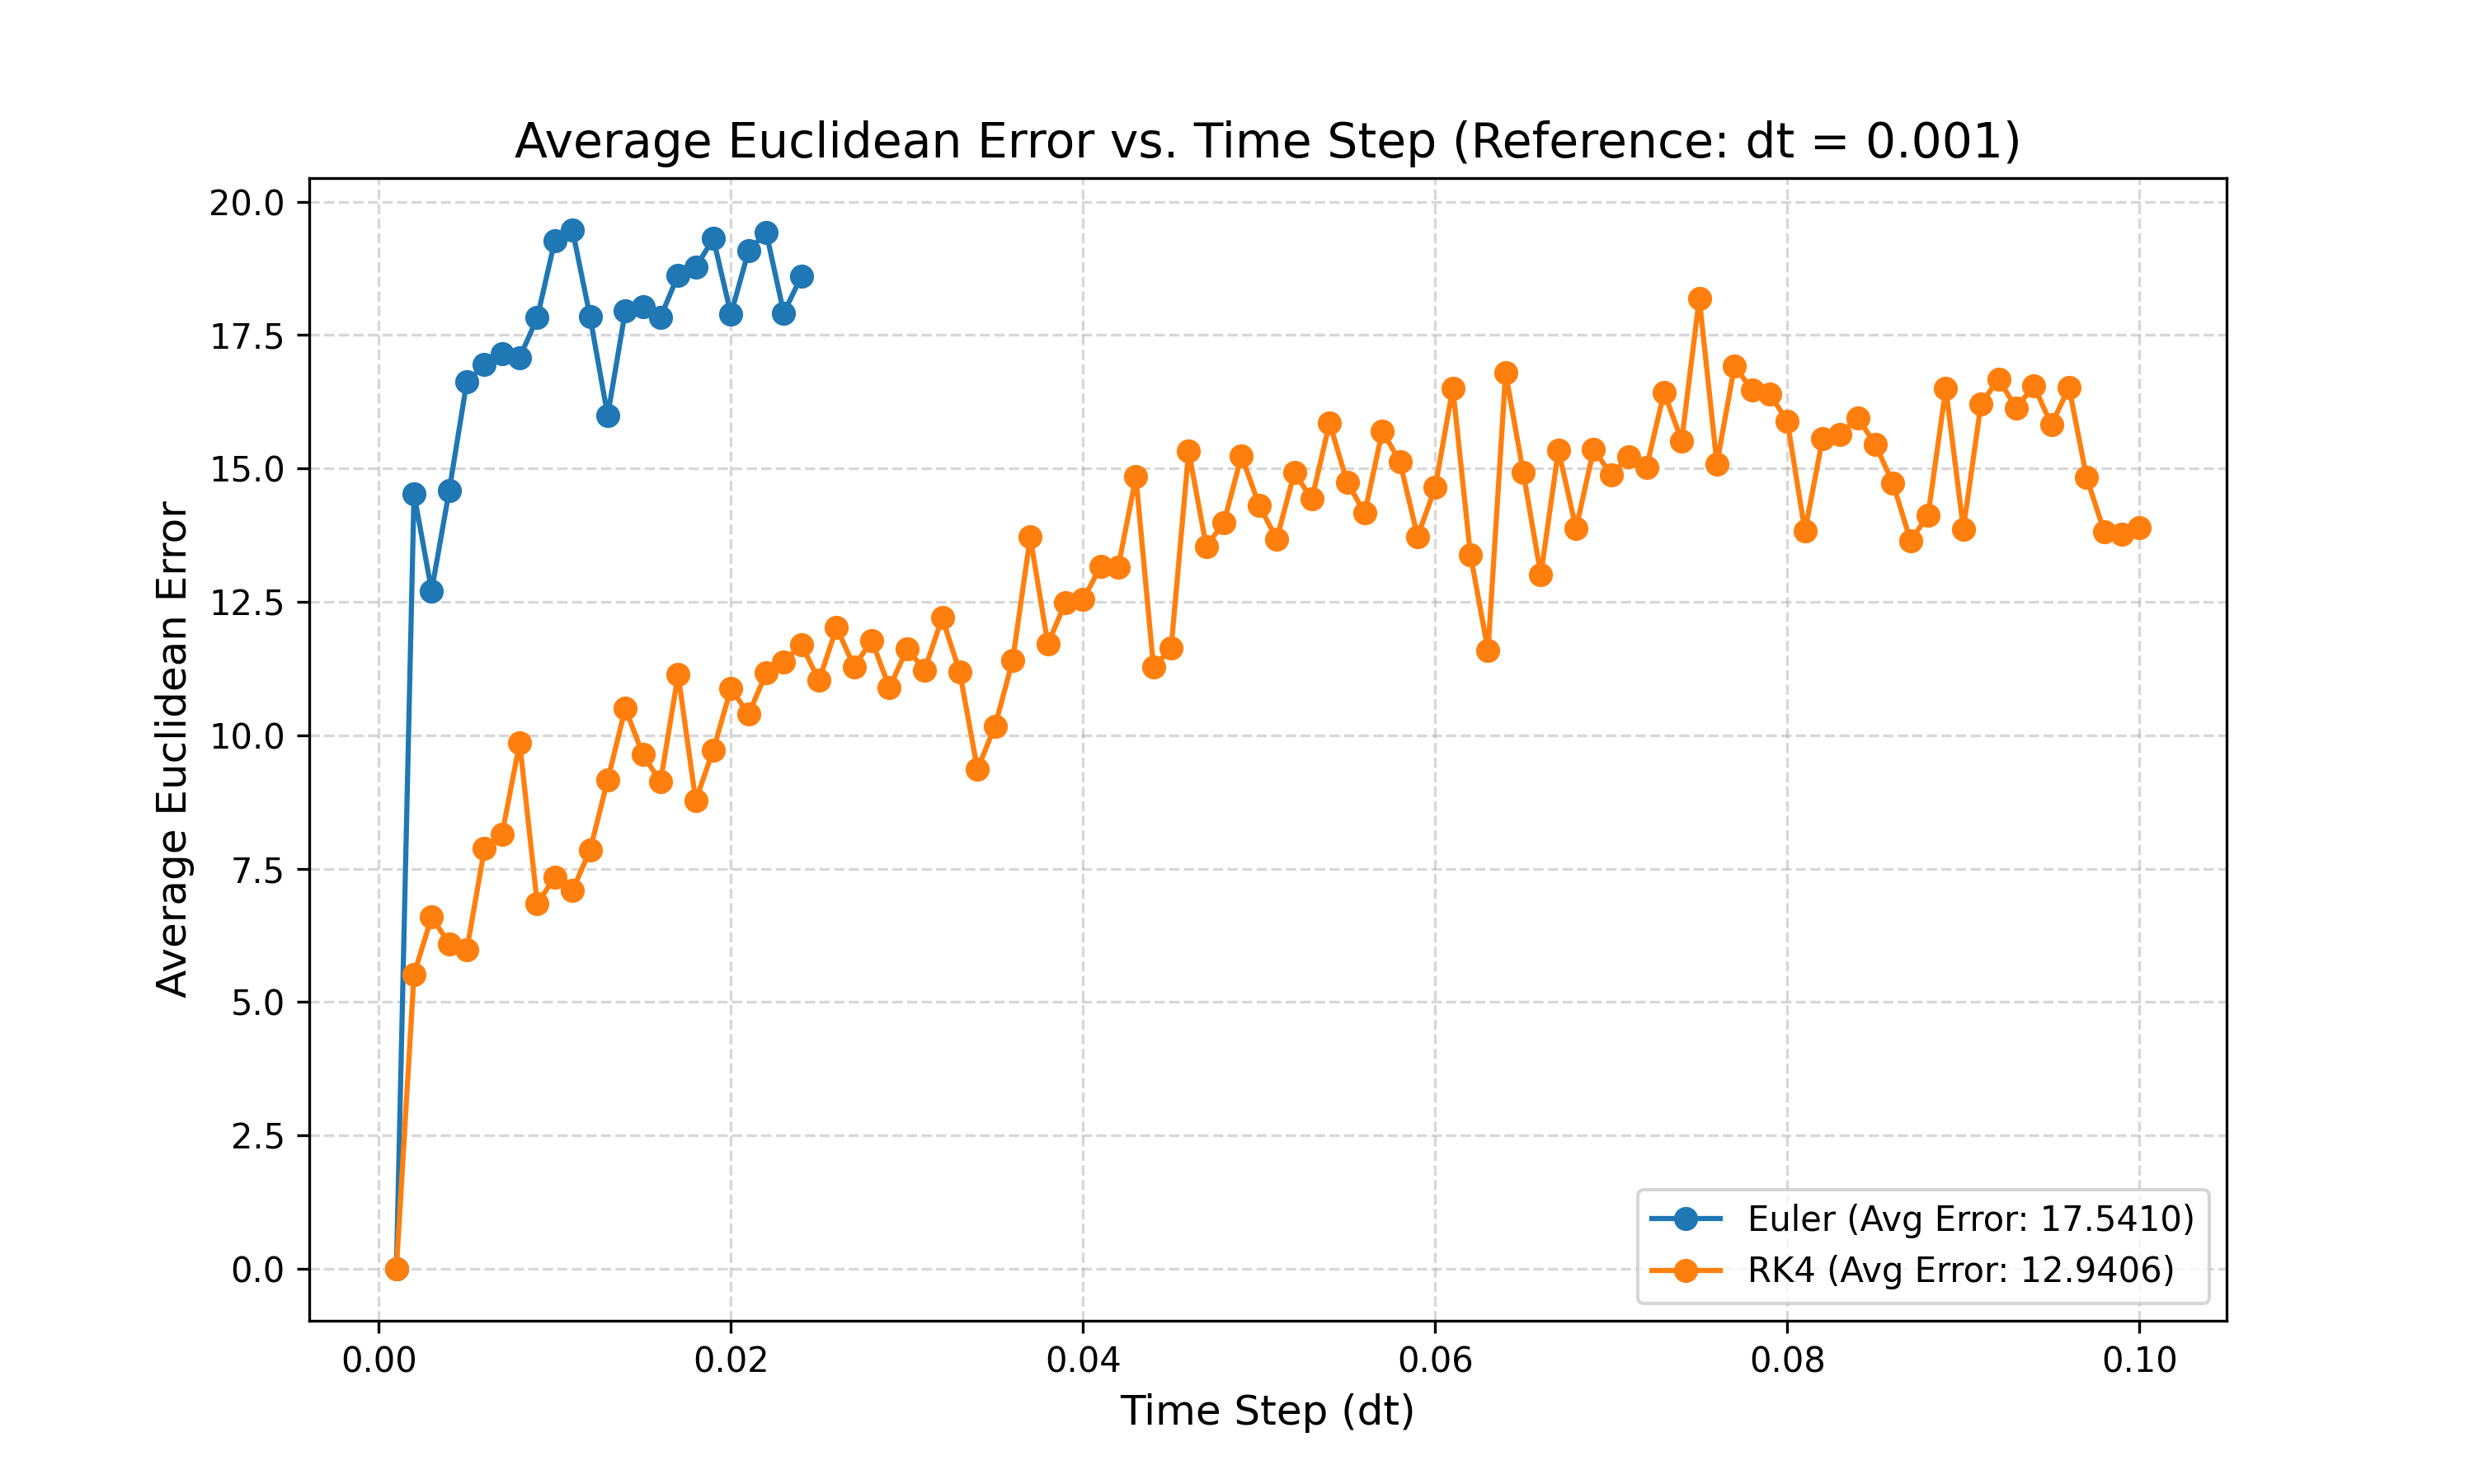
\includegraphics[width=0.9\linewidth]{images/error_comparison1000_114.png}
  \caption{Lorenz attractor error analysis with initial state \((1.0, 1.0, 1.0)\), using 1000 different time steps between \(10^{-3}\) and \(10^{-1}\), and a total simulation time of 40 seconds. For \(\Delta t > 0.025\), the Euler solution is not stable enough to reliably reproduce the attractor shape.
  \cite{youngaryanLorenzError1.1.41000_image}.}
  \label{fig:lorenz_error1000}
\end{figure}



\begin{figure}[!ht]
  \centering
  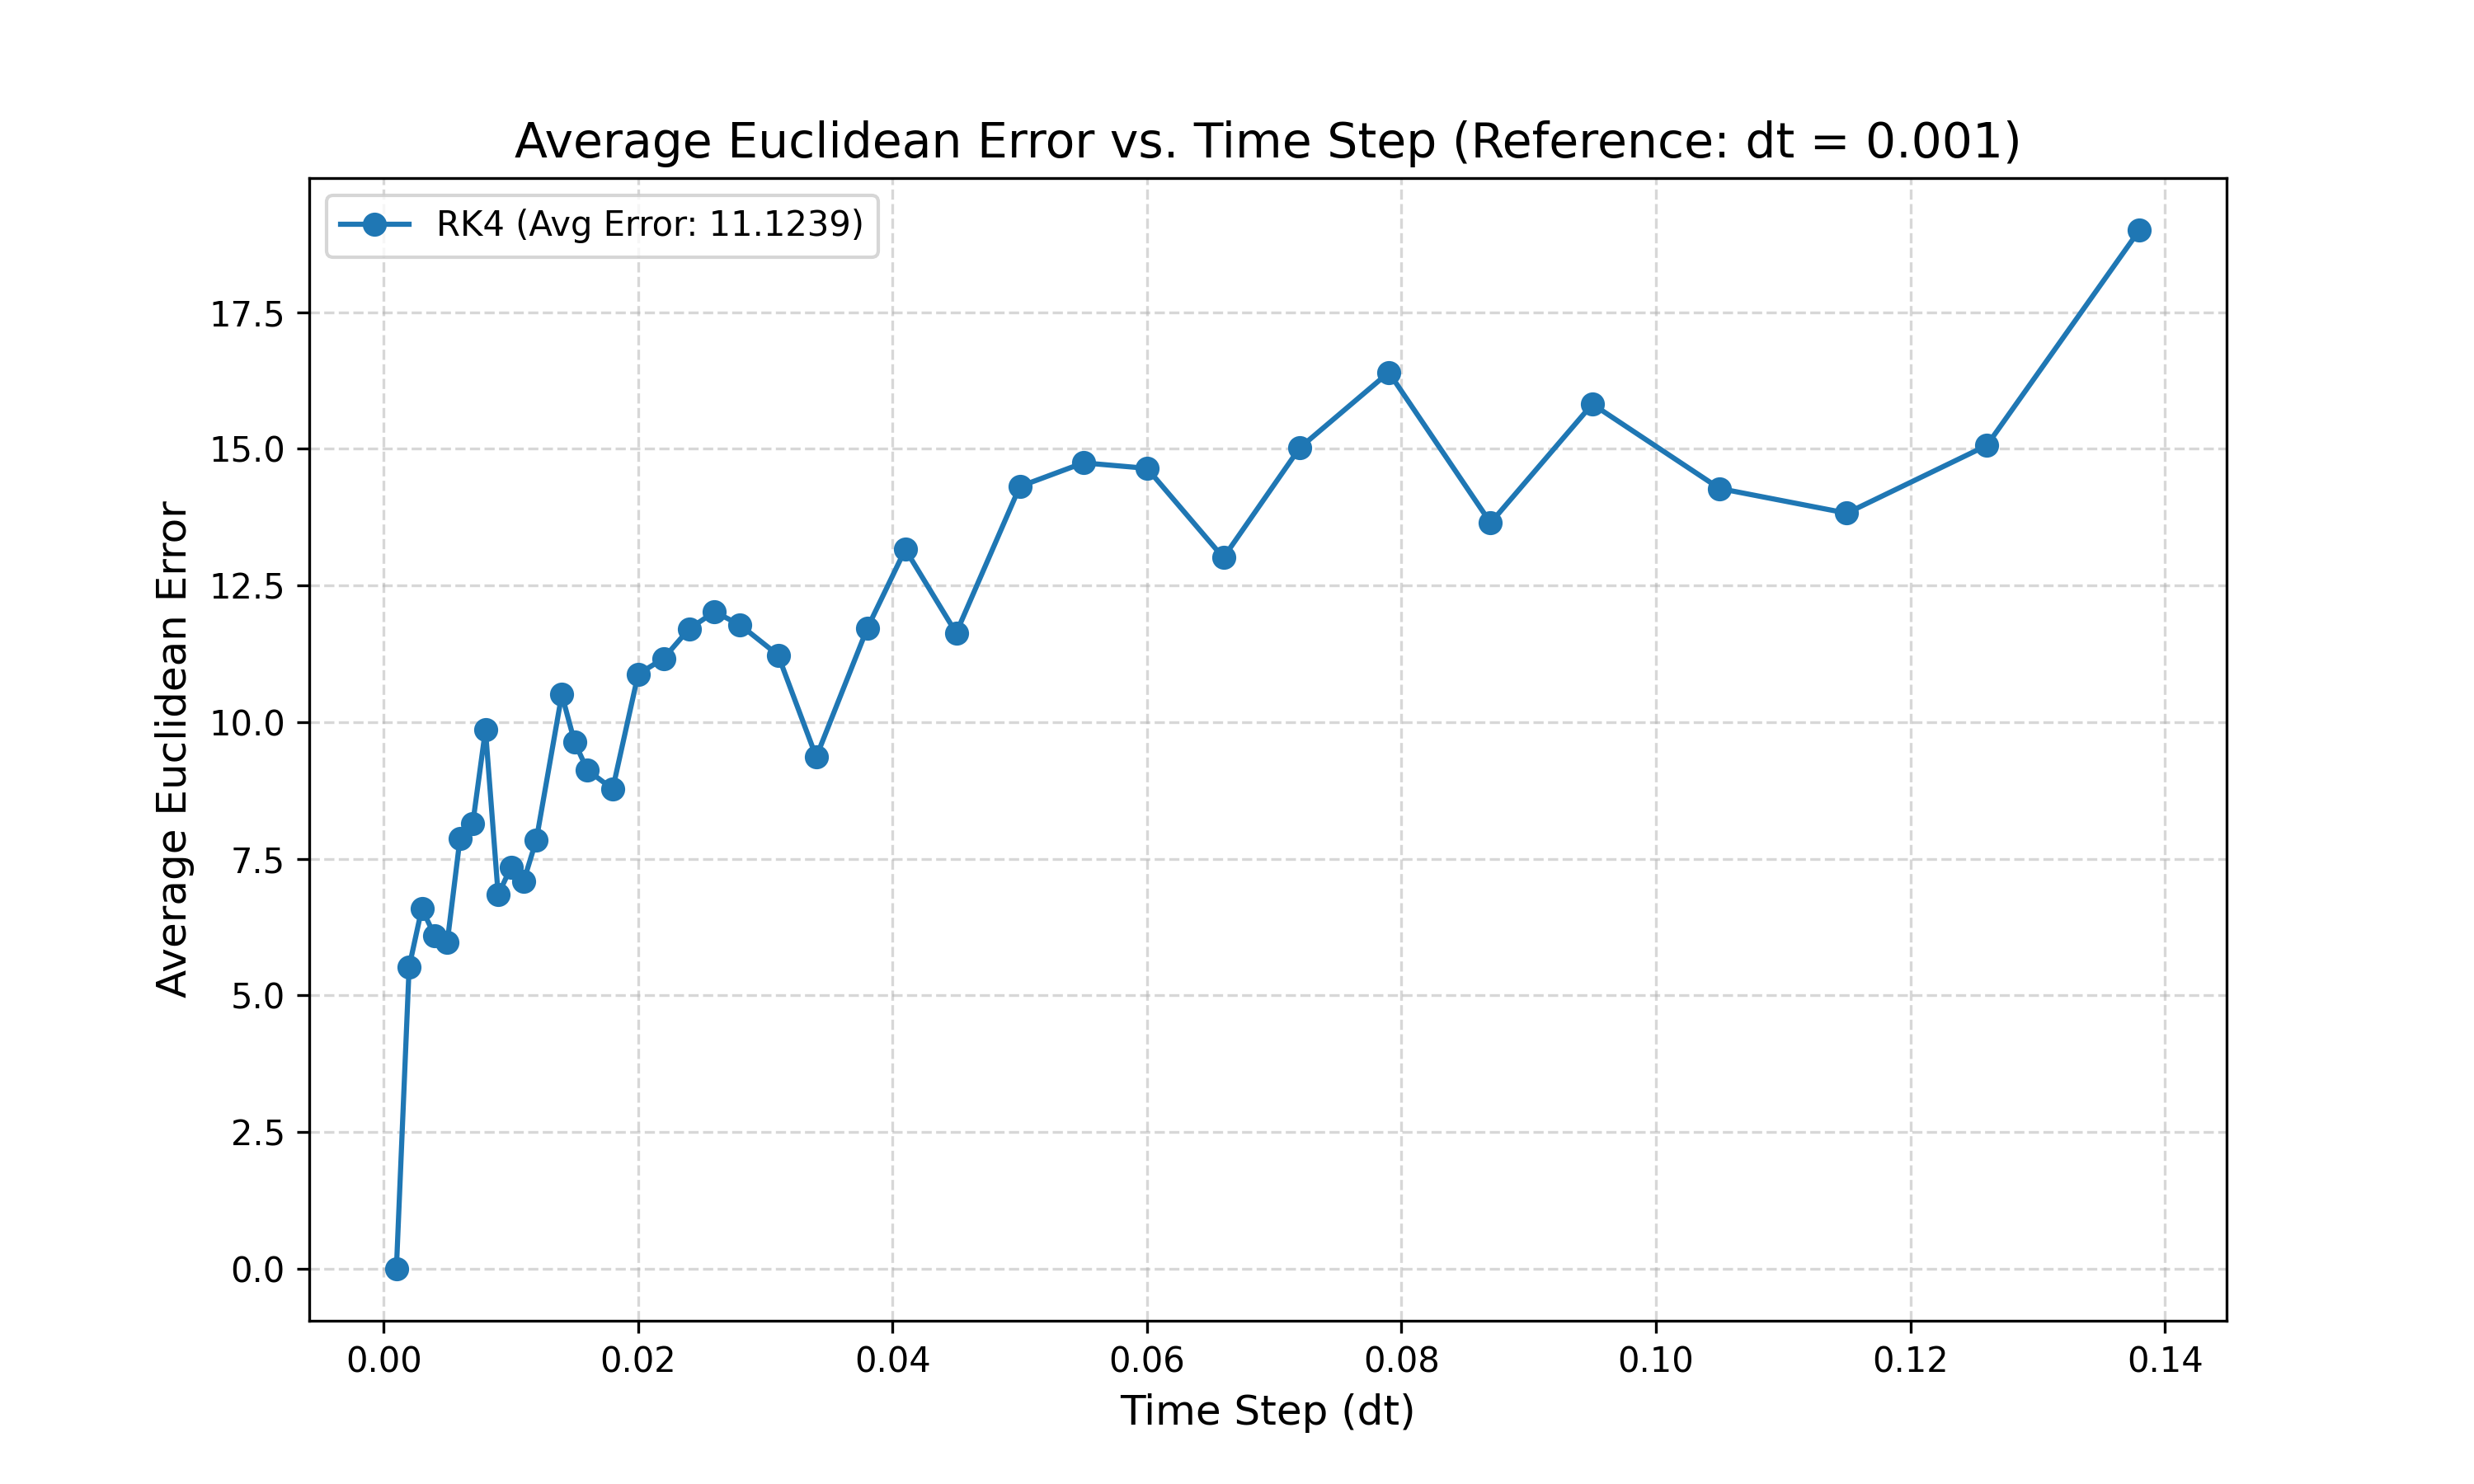
\includegraphics[width=0.9\linewidth]{images/error_comparison_rk4_stable_0.13.png}
  \caption{Lorenz attractor error analysis with initial state \((1.0, 1.0, 1.0)\), using 100 different time steps between \(10^{-3}\) and \(10^{1}\), and a total simulation time of 40 seconds. For \(\Delta t < 0.14\), the RK4 solution is stable enough to  reproduce the attractor shape. \cite{youngaryanerror_comparison_rk4_stable_0.13sCode}.}
  \label{fig:error_comparison_rk4_stable_0.13}
\end{figure}

\begin{figure}[!ht]
  \centering
  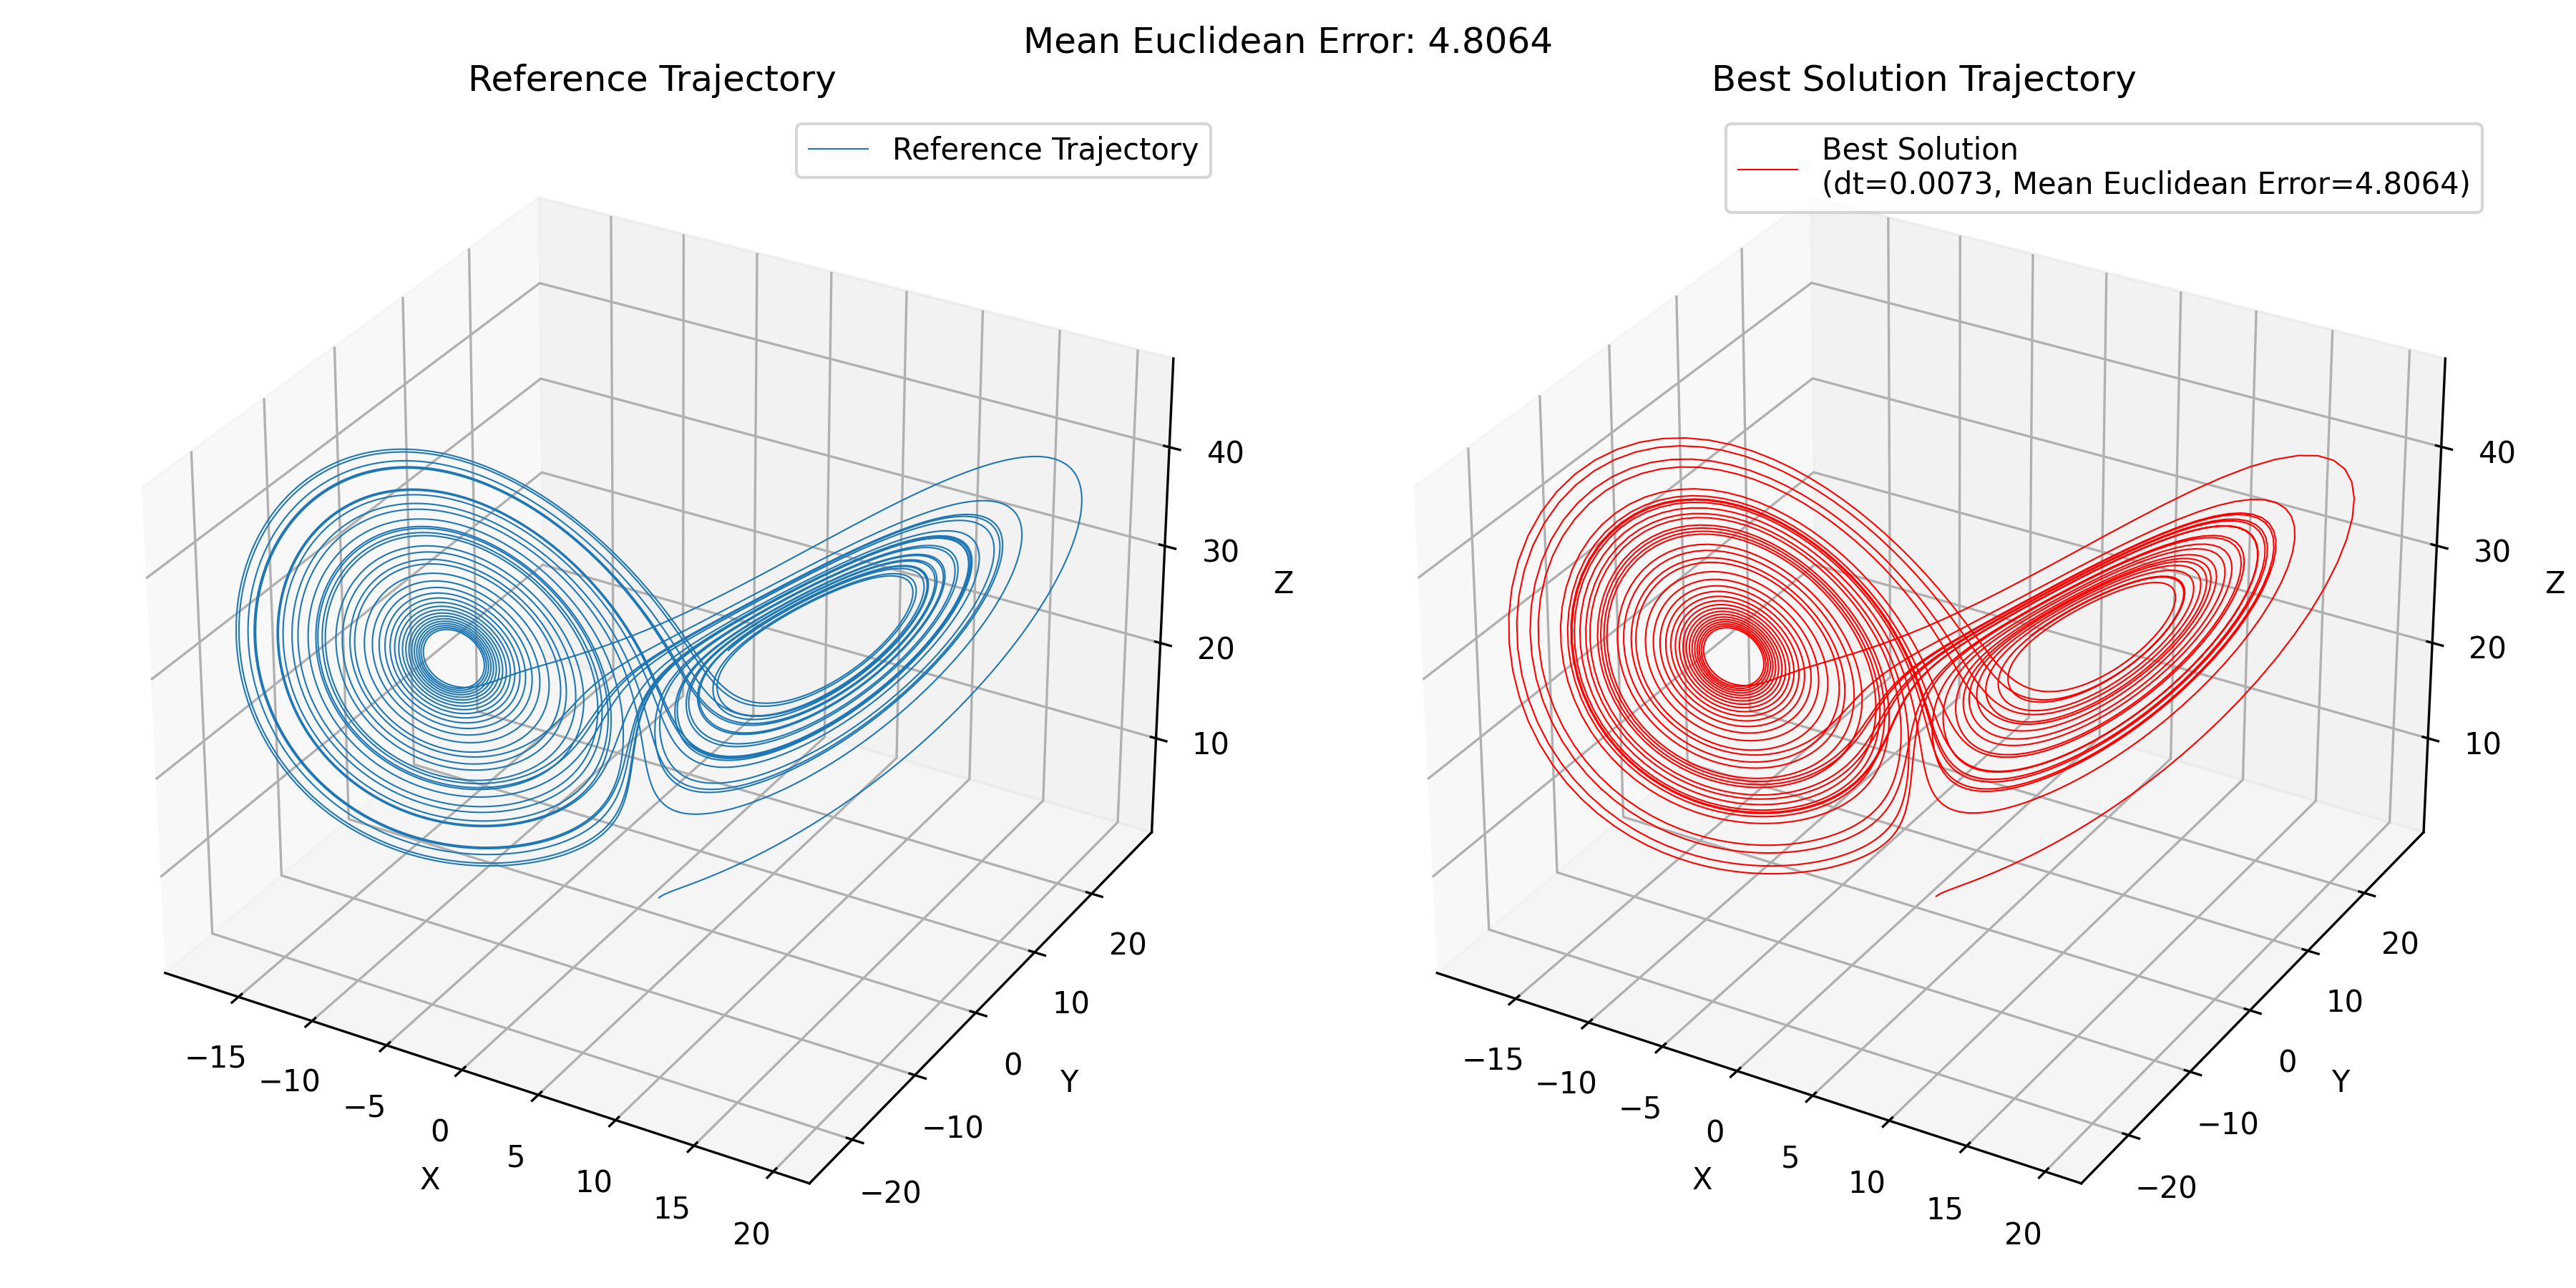
\includegraphics[width=0.9\linewidth]{images/optuna_lorenz_3d.png}
  \caption{Comparison between reference system with \(\Delta t = 0.001\) and a less computationally expensive system with step size of \(\Delta t = 0.0073\), for this I used Optuna \cite{akiba2019optuna} with 50 trials. the code is at \cite{youngaryanOptunaCode} and the image \cite{youngaryanoptunaComparisonImage}.}
  \label{fig:optuna_lorenz_3d}
\end{figure}


\begin{figure}[!ht]
  \centering
  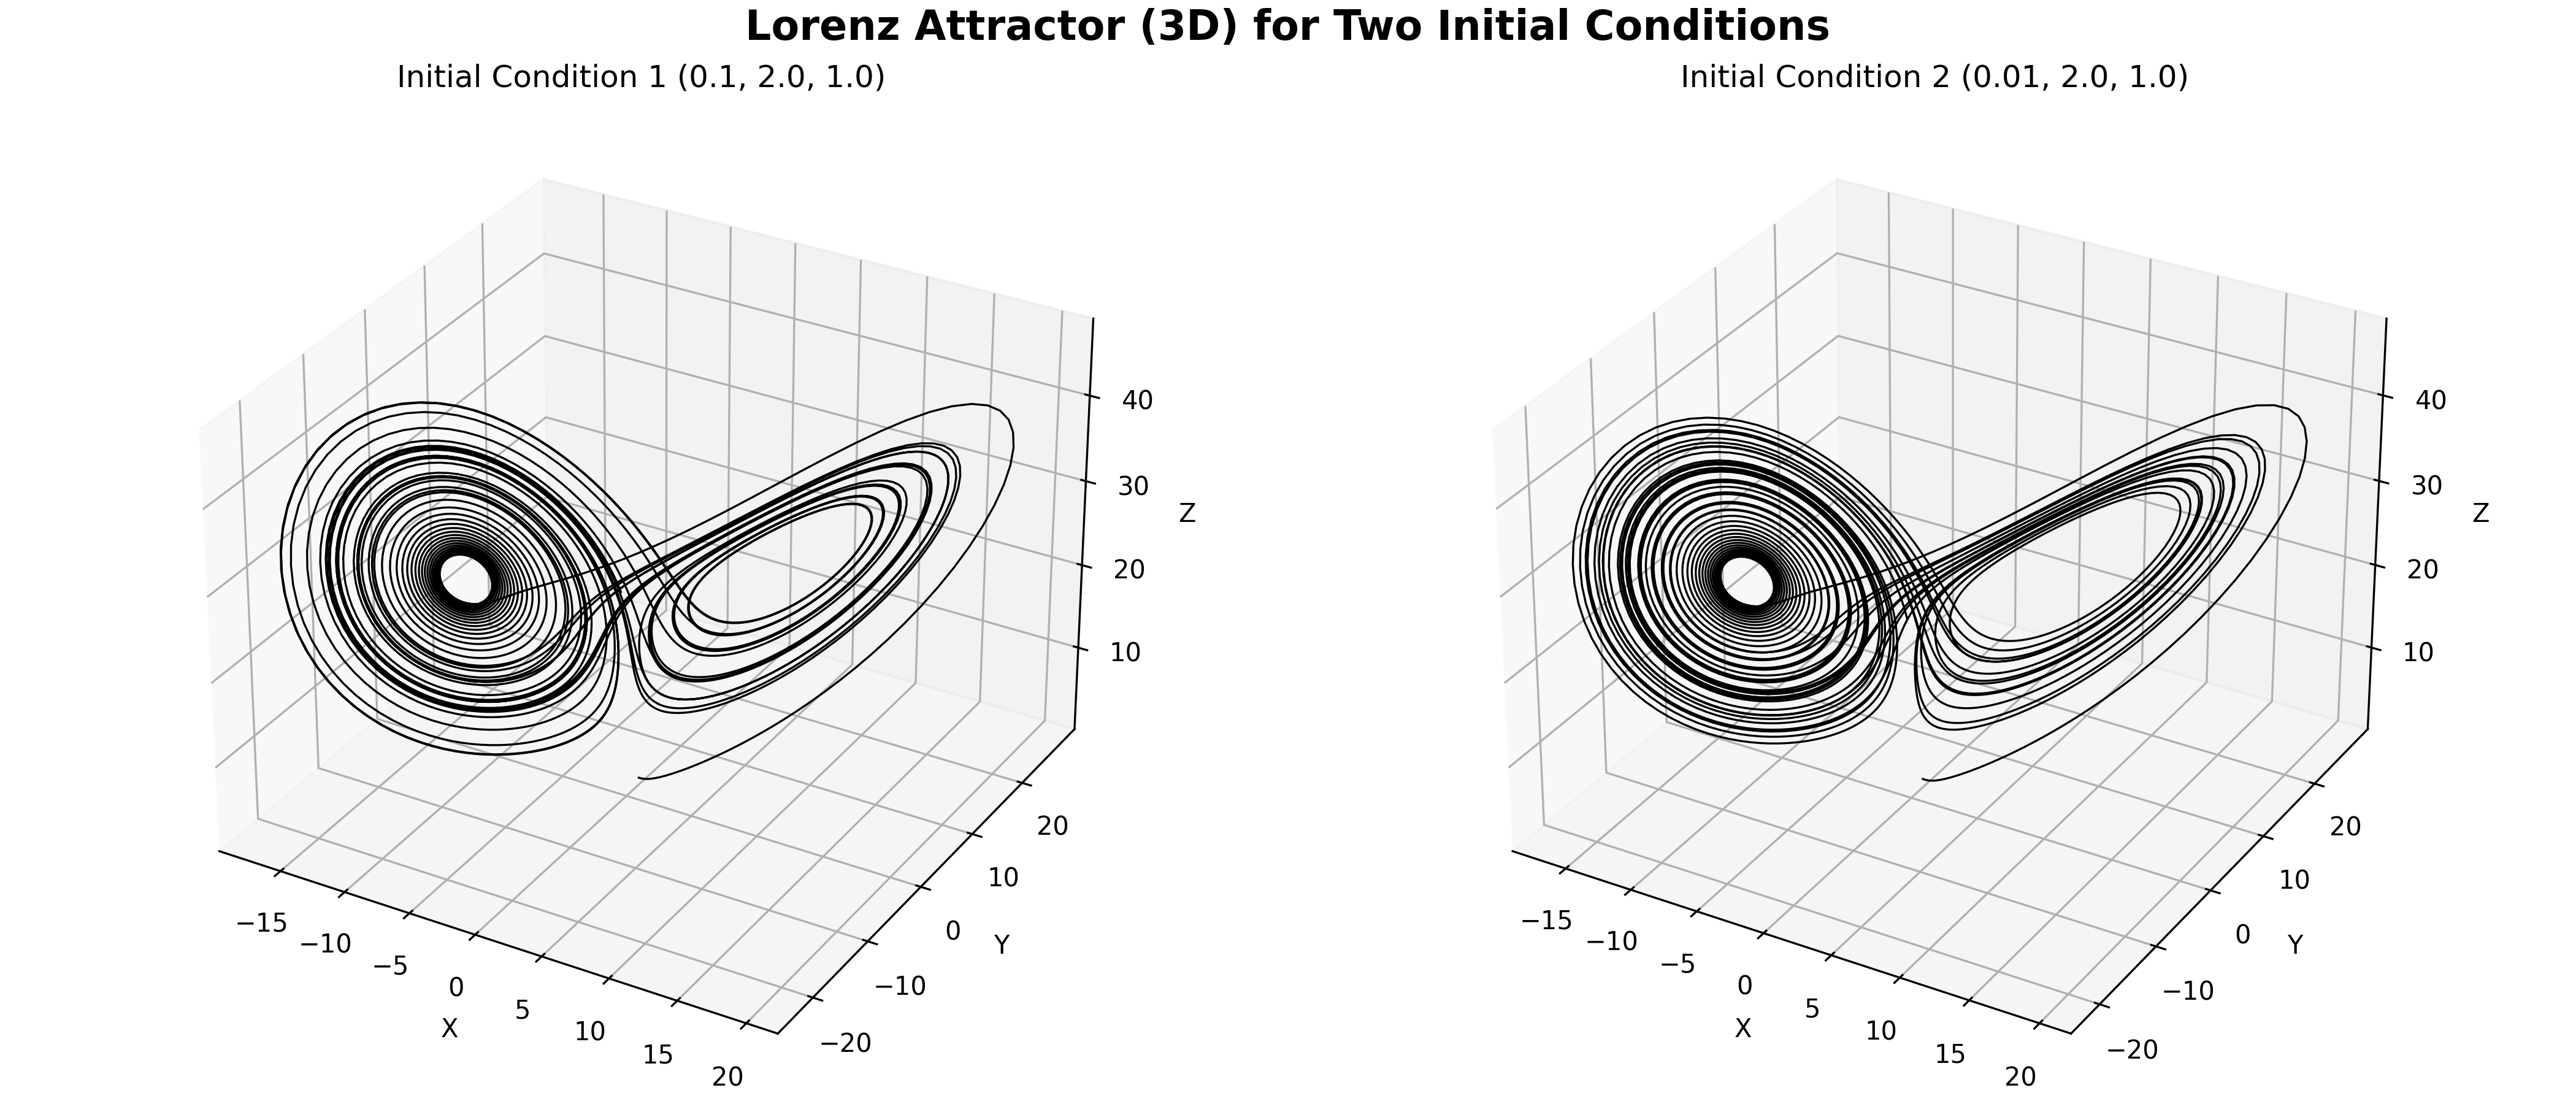
\includegraphics[width=0.9\linewidth]{images/two_initial_conditions_3d_separate.png}
  \caption{Comparison between two similar initial conditions of (0.01, 2.0, 1.0) and (0.1, 2.0, 1.0) and
  the time steps of $\Delta t = 0.0073$ to show the chaotic behavior of the system. the code is at \cite{youngaryantwo_initial_conditions_3d_separateICode} and the image \cite{youngaryantwo_initial_conditions_3d_separateImg}.}
  \label{fig:two_initial_conditions_3d_separate}
\end{figure}


\begin{figure}[!ht]
  \centering
  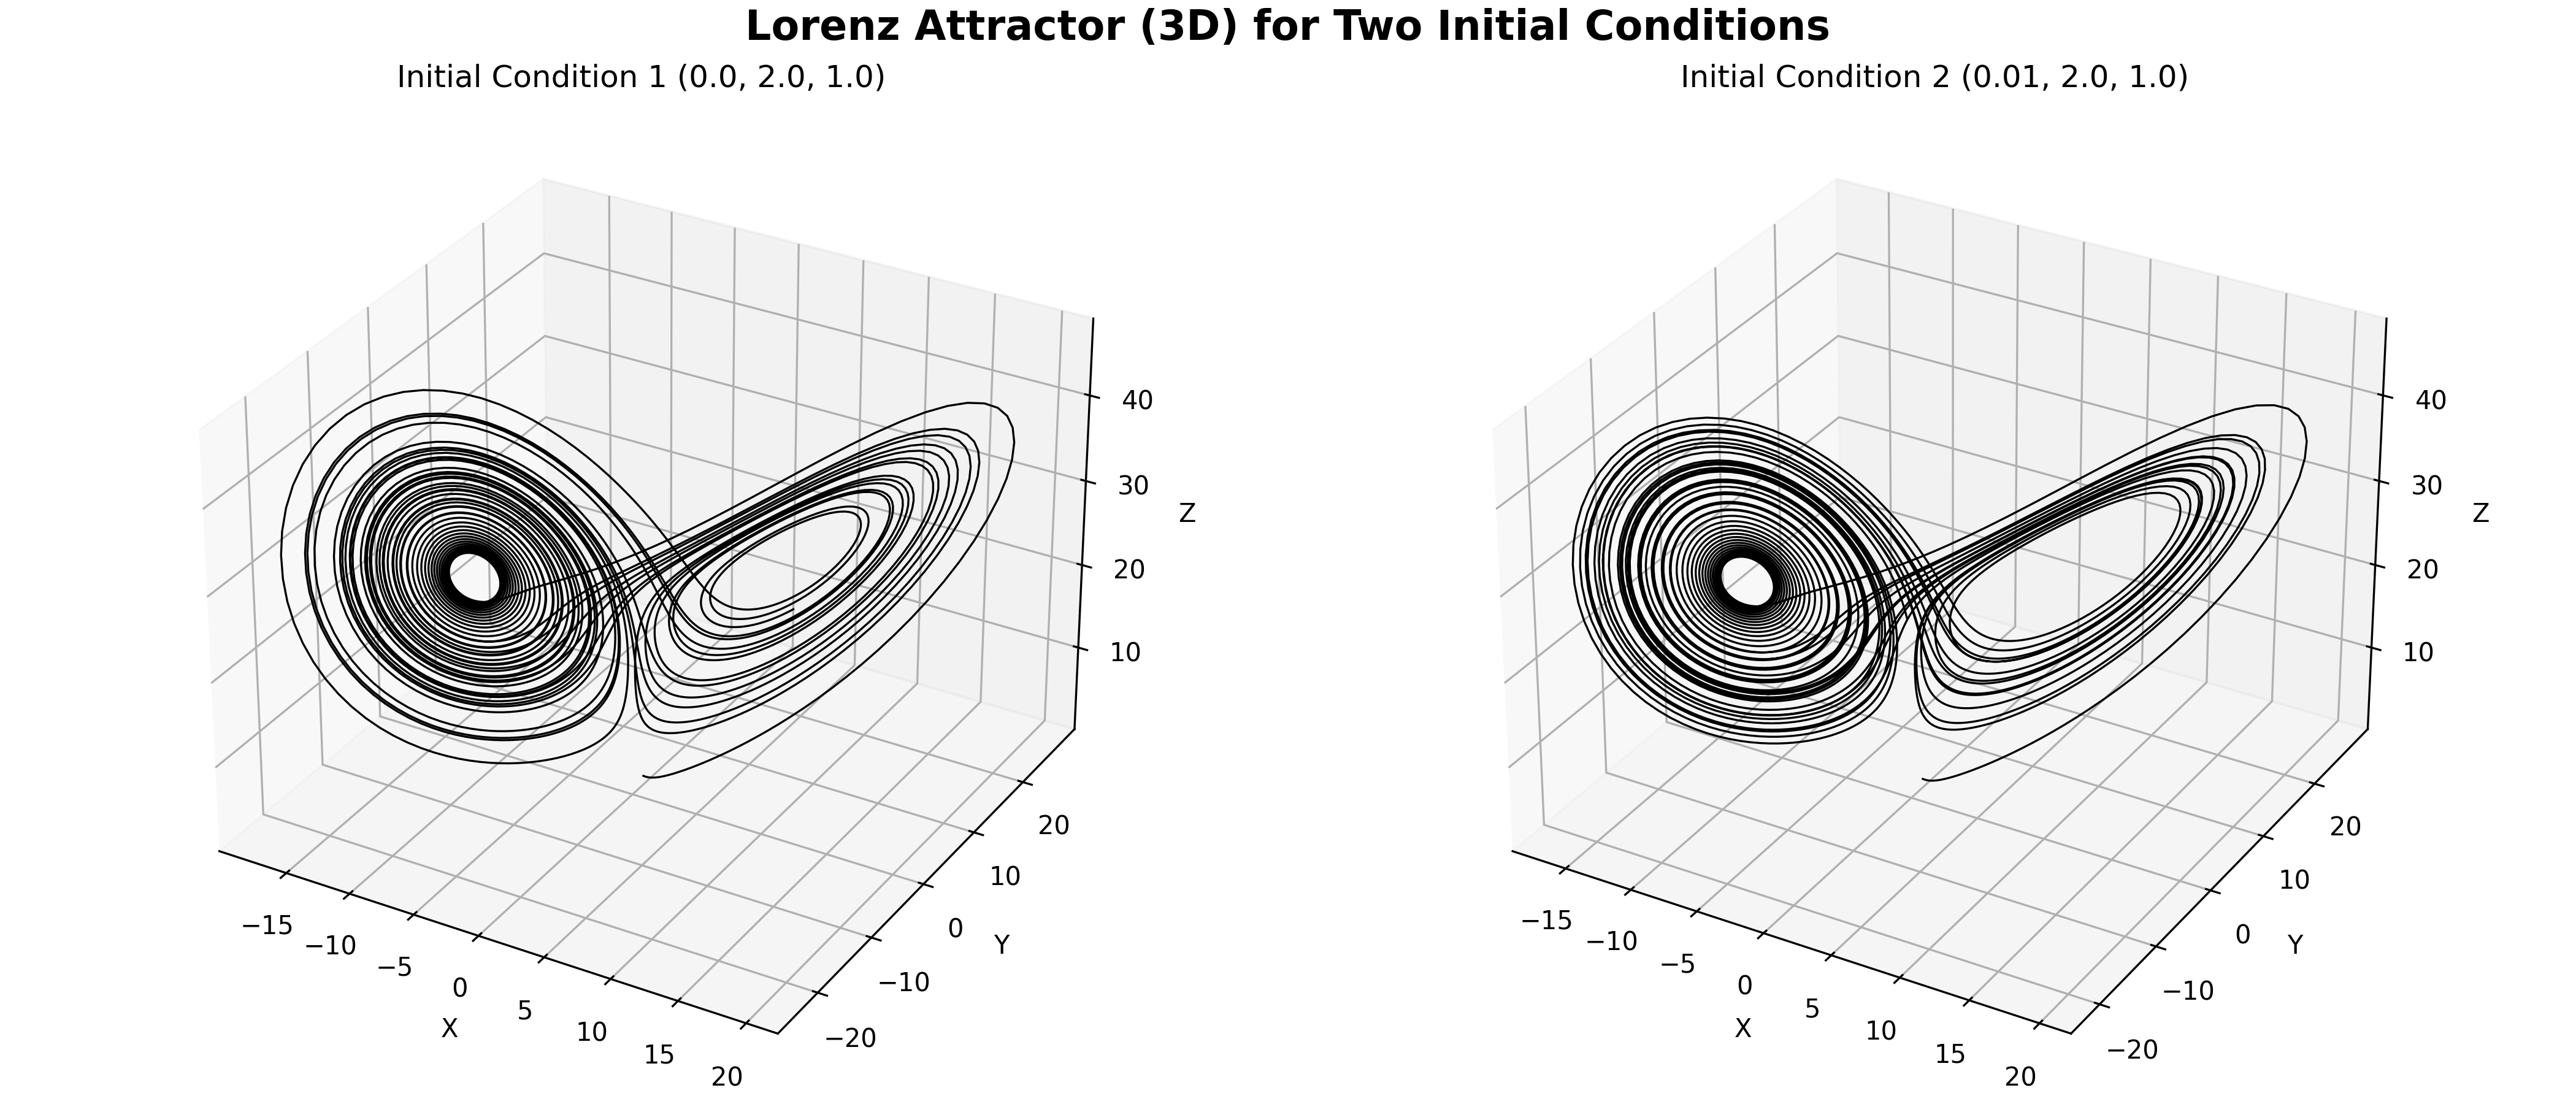
\includegraphics[width=0.9\linewidth]{images/two_initial_conditions_3d_separate_2.png}
  \caption{Comparison between two similar initial conditions of (0.0, 2.0, 1.0) and (0.1, 2.0, 1.0) and
the time steps of $\Delta t = 0.0073$ to show the chaotic behavior of the system. the code is at \cite{youngaryantwo_initial_conditions_3d_separateICode} and the image \cite{youngaryantwo_initial_conditions_3d_2separateICode}.}
  \label{fig:two_initial_conditions_3d_separate_2}
\end{figure}

\begin{figure}[!ht]
  \centering
  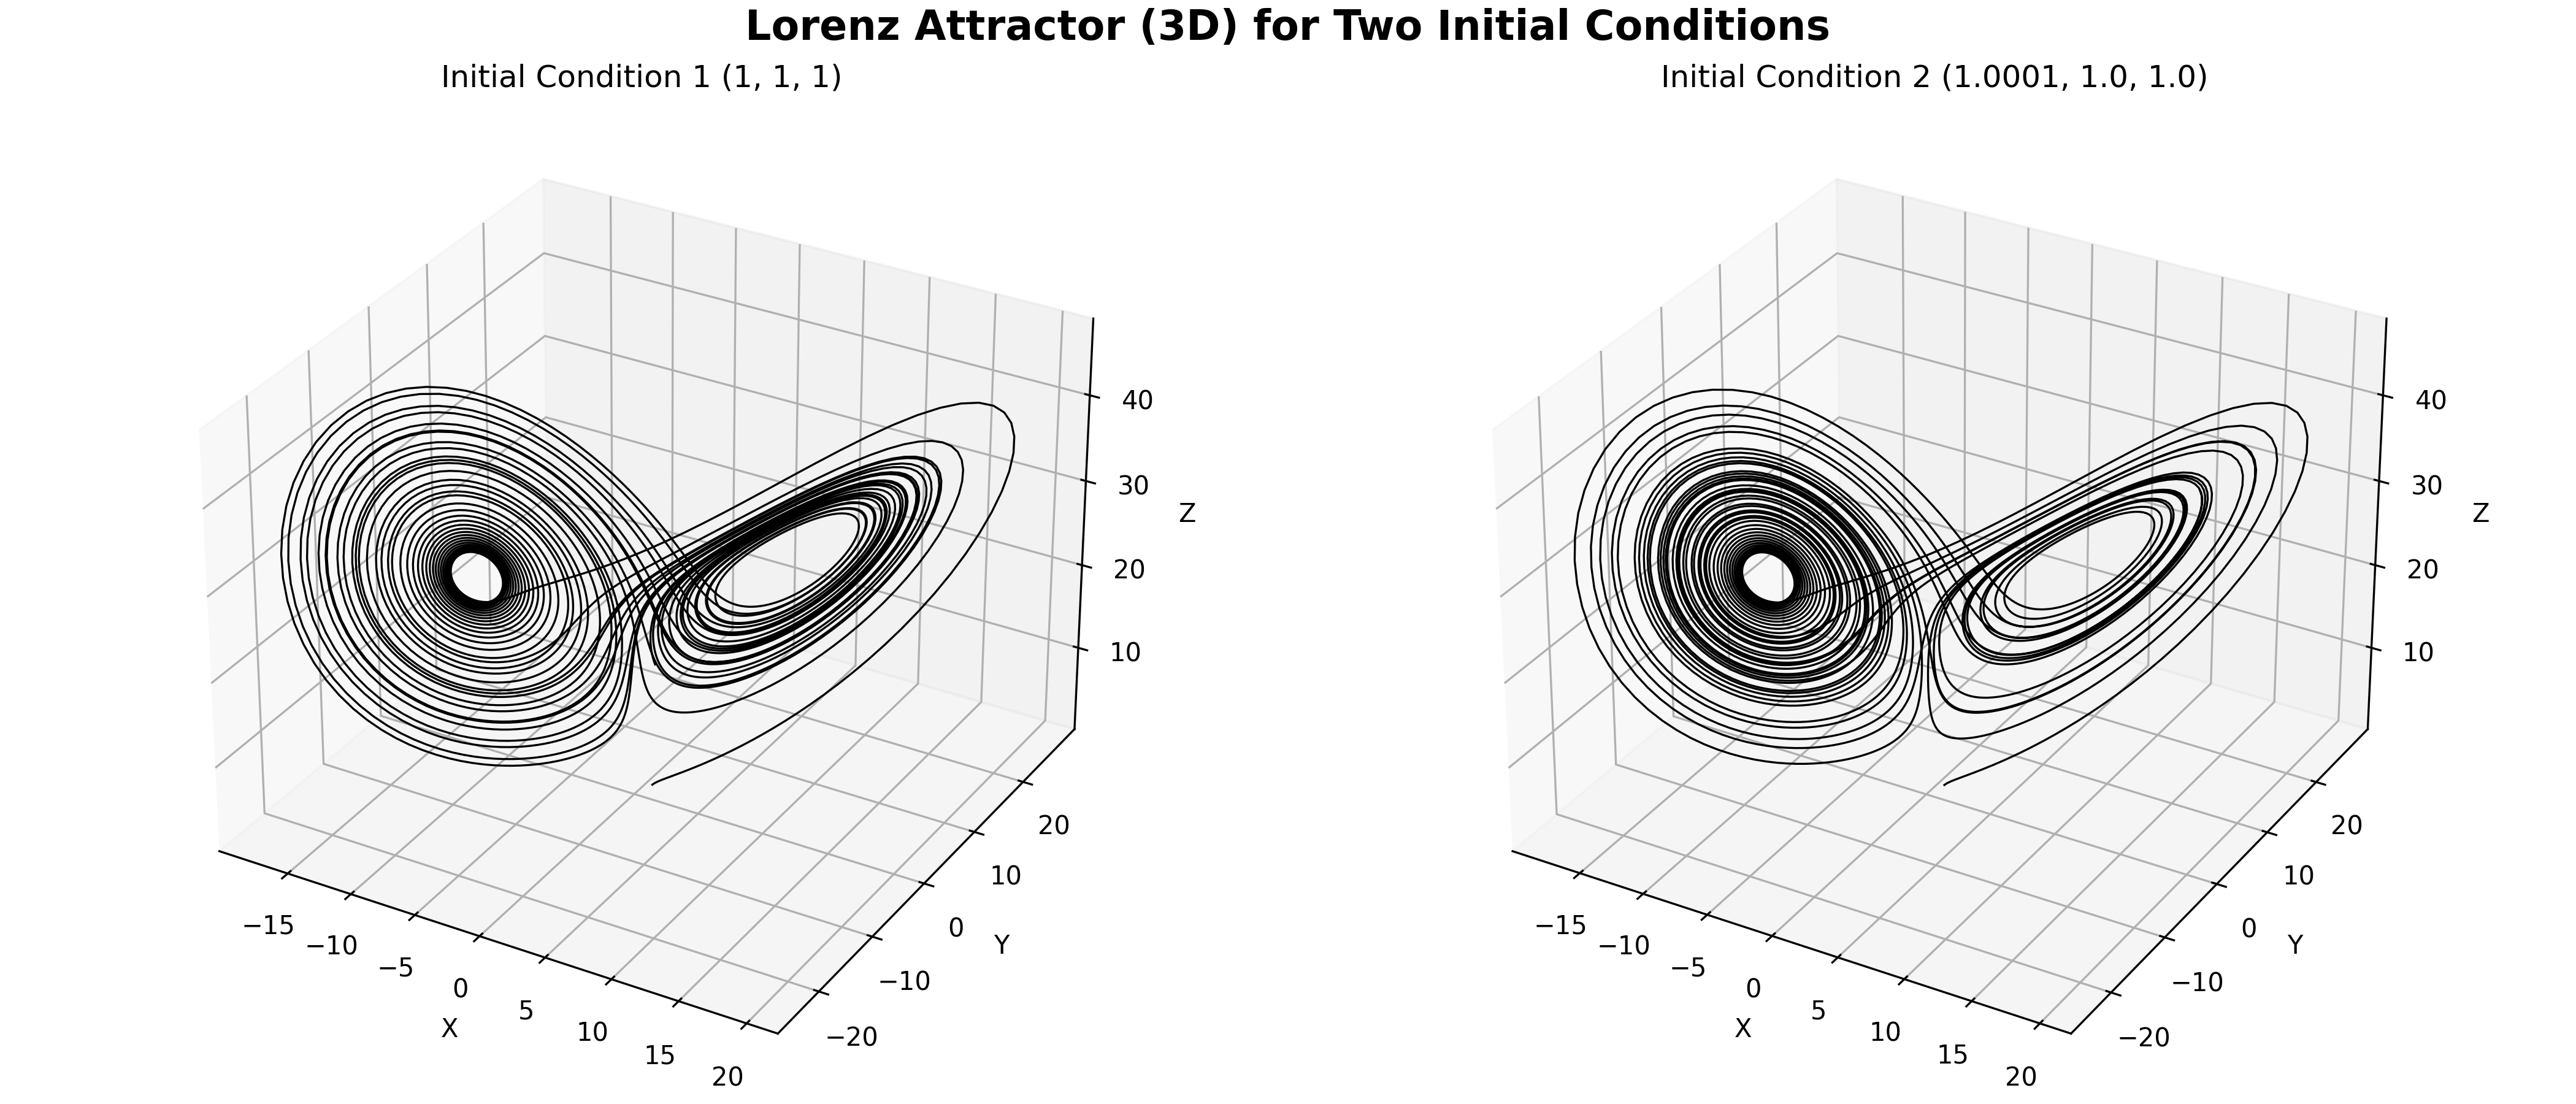
\includegraphics[width=0.9\linewidth]{images/two_initial_conditions_3d_separate_3.png}
  \caption{Comparison between two similar initial conditions of (1.0, 1.0, 1.0) and (1.0001, 1.0, 1.0) and
the time steps of$\Delta t = 0.0073$ to show the chaotic behavior of the system. the code is at \cite{youngaryantwo_initial_conditions_3d_separateICode} and the image \cite{youngaryantwo_initial_conditions_3d_3separateICode}.}
  \label{fig:two_initial_conditions_3d_separate_3}
\end{figure}



\begin{figure}[!ht]
  \centering
  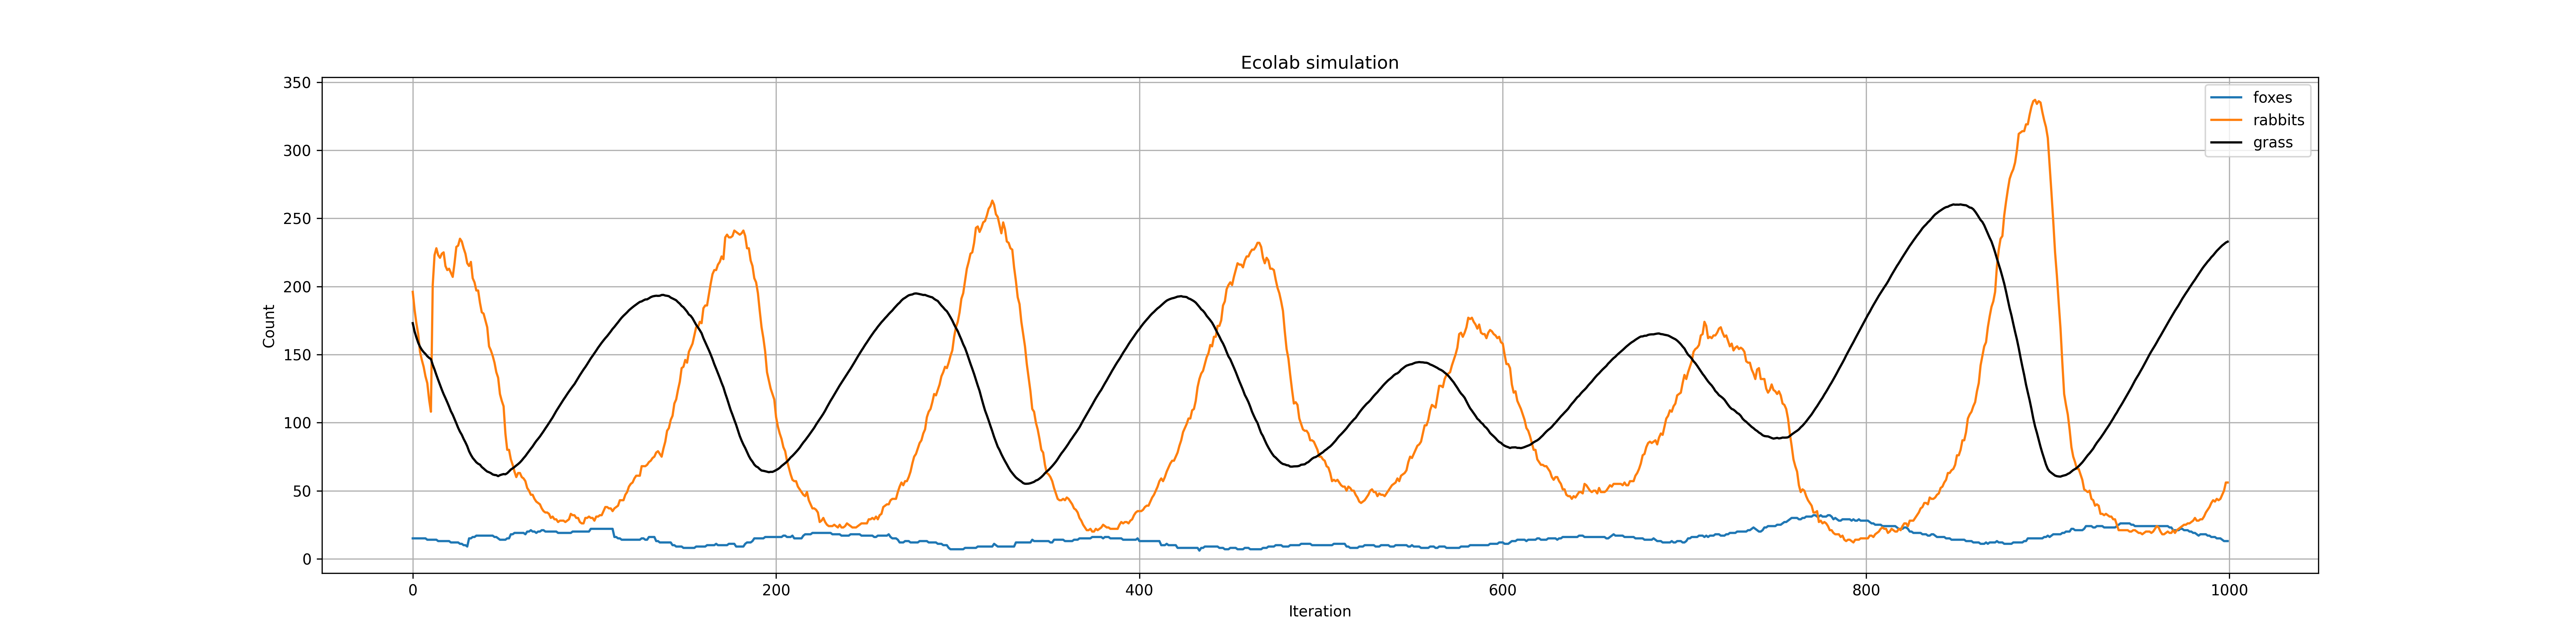
\includegraphics[width=0.9\linewidth]{images/Ecolab_simulation.png}
  \caption{Simulation of a prey-predator system with the following initial settings: \texttt{Environment(shape=[60,60], growrate=60, maxgrass=50, startgrass=1)}, \texttt{Nrabbits = 200}, \texttt{Nfoxes = 15}. Rabbits are initialized with \texttt{speed=1}, \texttt{vision=5}, \texttt{breedfreq=10}, \texttt{breedfood=10}, and \texttt{maxage=40}. Foxes are initialized with \texttt{speed=3}, \texttt{vision=7}, \texttt{breedfreq=30}, \texttt{breedfood=20}, and \texttt{maxage=80}. See \cite{youngaryantwo_initial_conditions_3d_separateICode} for code and \cite{youngaryantwo_initial_conditions_3d_3separateICode} for the source image.}
  \label{fig:Ecolab_pred_prey}
\end{figure}


\begin{figure}[!ht]
  \centering
  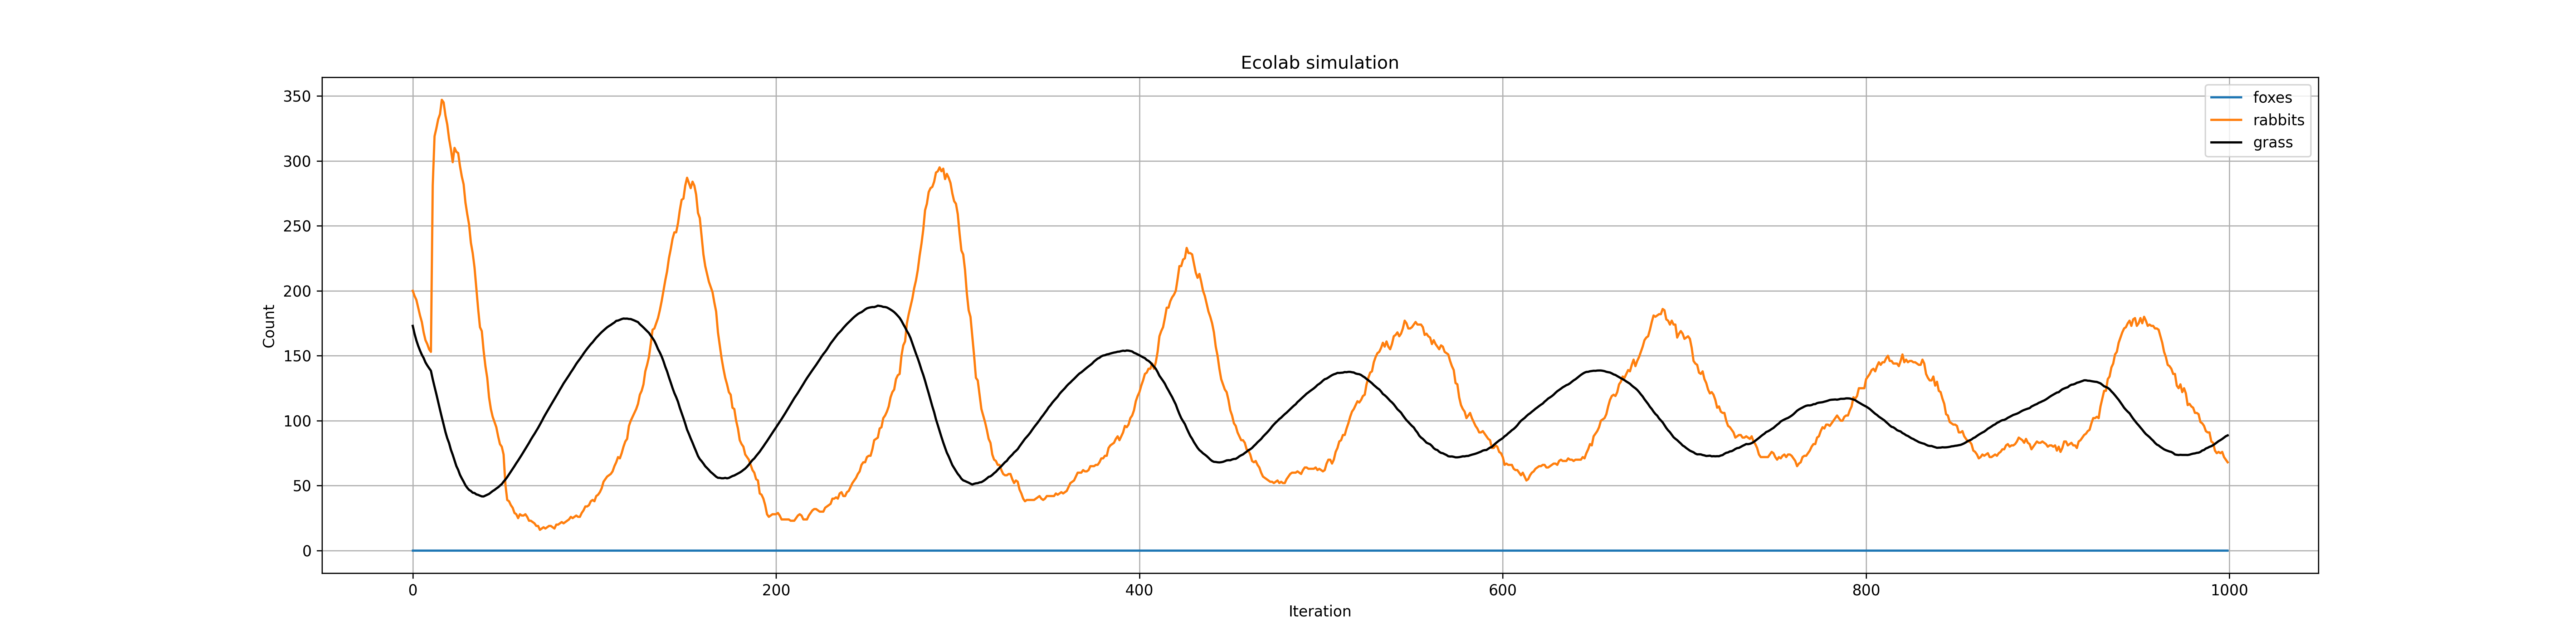
\includegraphics[width=0.9\linewidth]{images/Ecolab_simulation_no_foxes.png}
  \caption{Simulation of a prey-predator system with the following initial settings: \texttt{Environment(shape=[60,60], growrate=60, maxgrass=50, startgrass=1)}, \texttt{Nrabbits = 200}, \texttt{Nfoxes = 15}. Rabbits are initialized with \texttt{speed=1}, \texttt{vision=5}, \texttt{breedfreq=10}, \texttt{breedfood=10}, and \texttt{maxage=40}. And ero foxes. See \cite{youngaryantwo_initial_conditions_3d_separateICode} for code and \cite{youngaryantwo_initial_conditions_3d_3separateICode} for the source image.}
  \label{fig:Ecolab_pred_prey_no_foxes}
\end{figure}


\begin{figure}[!ht]
  \centering
  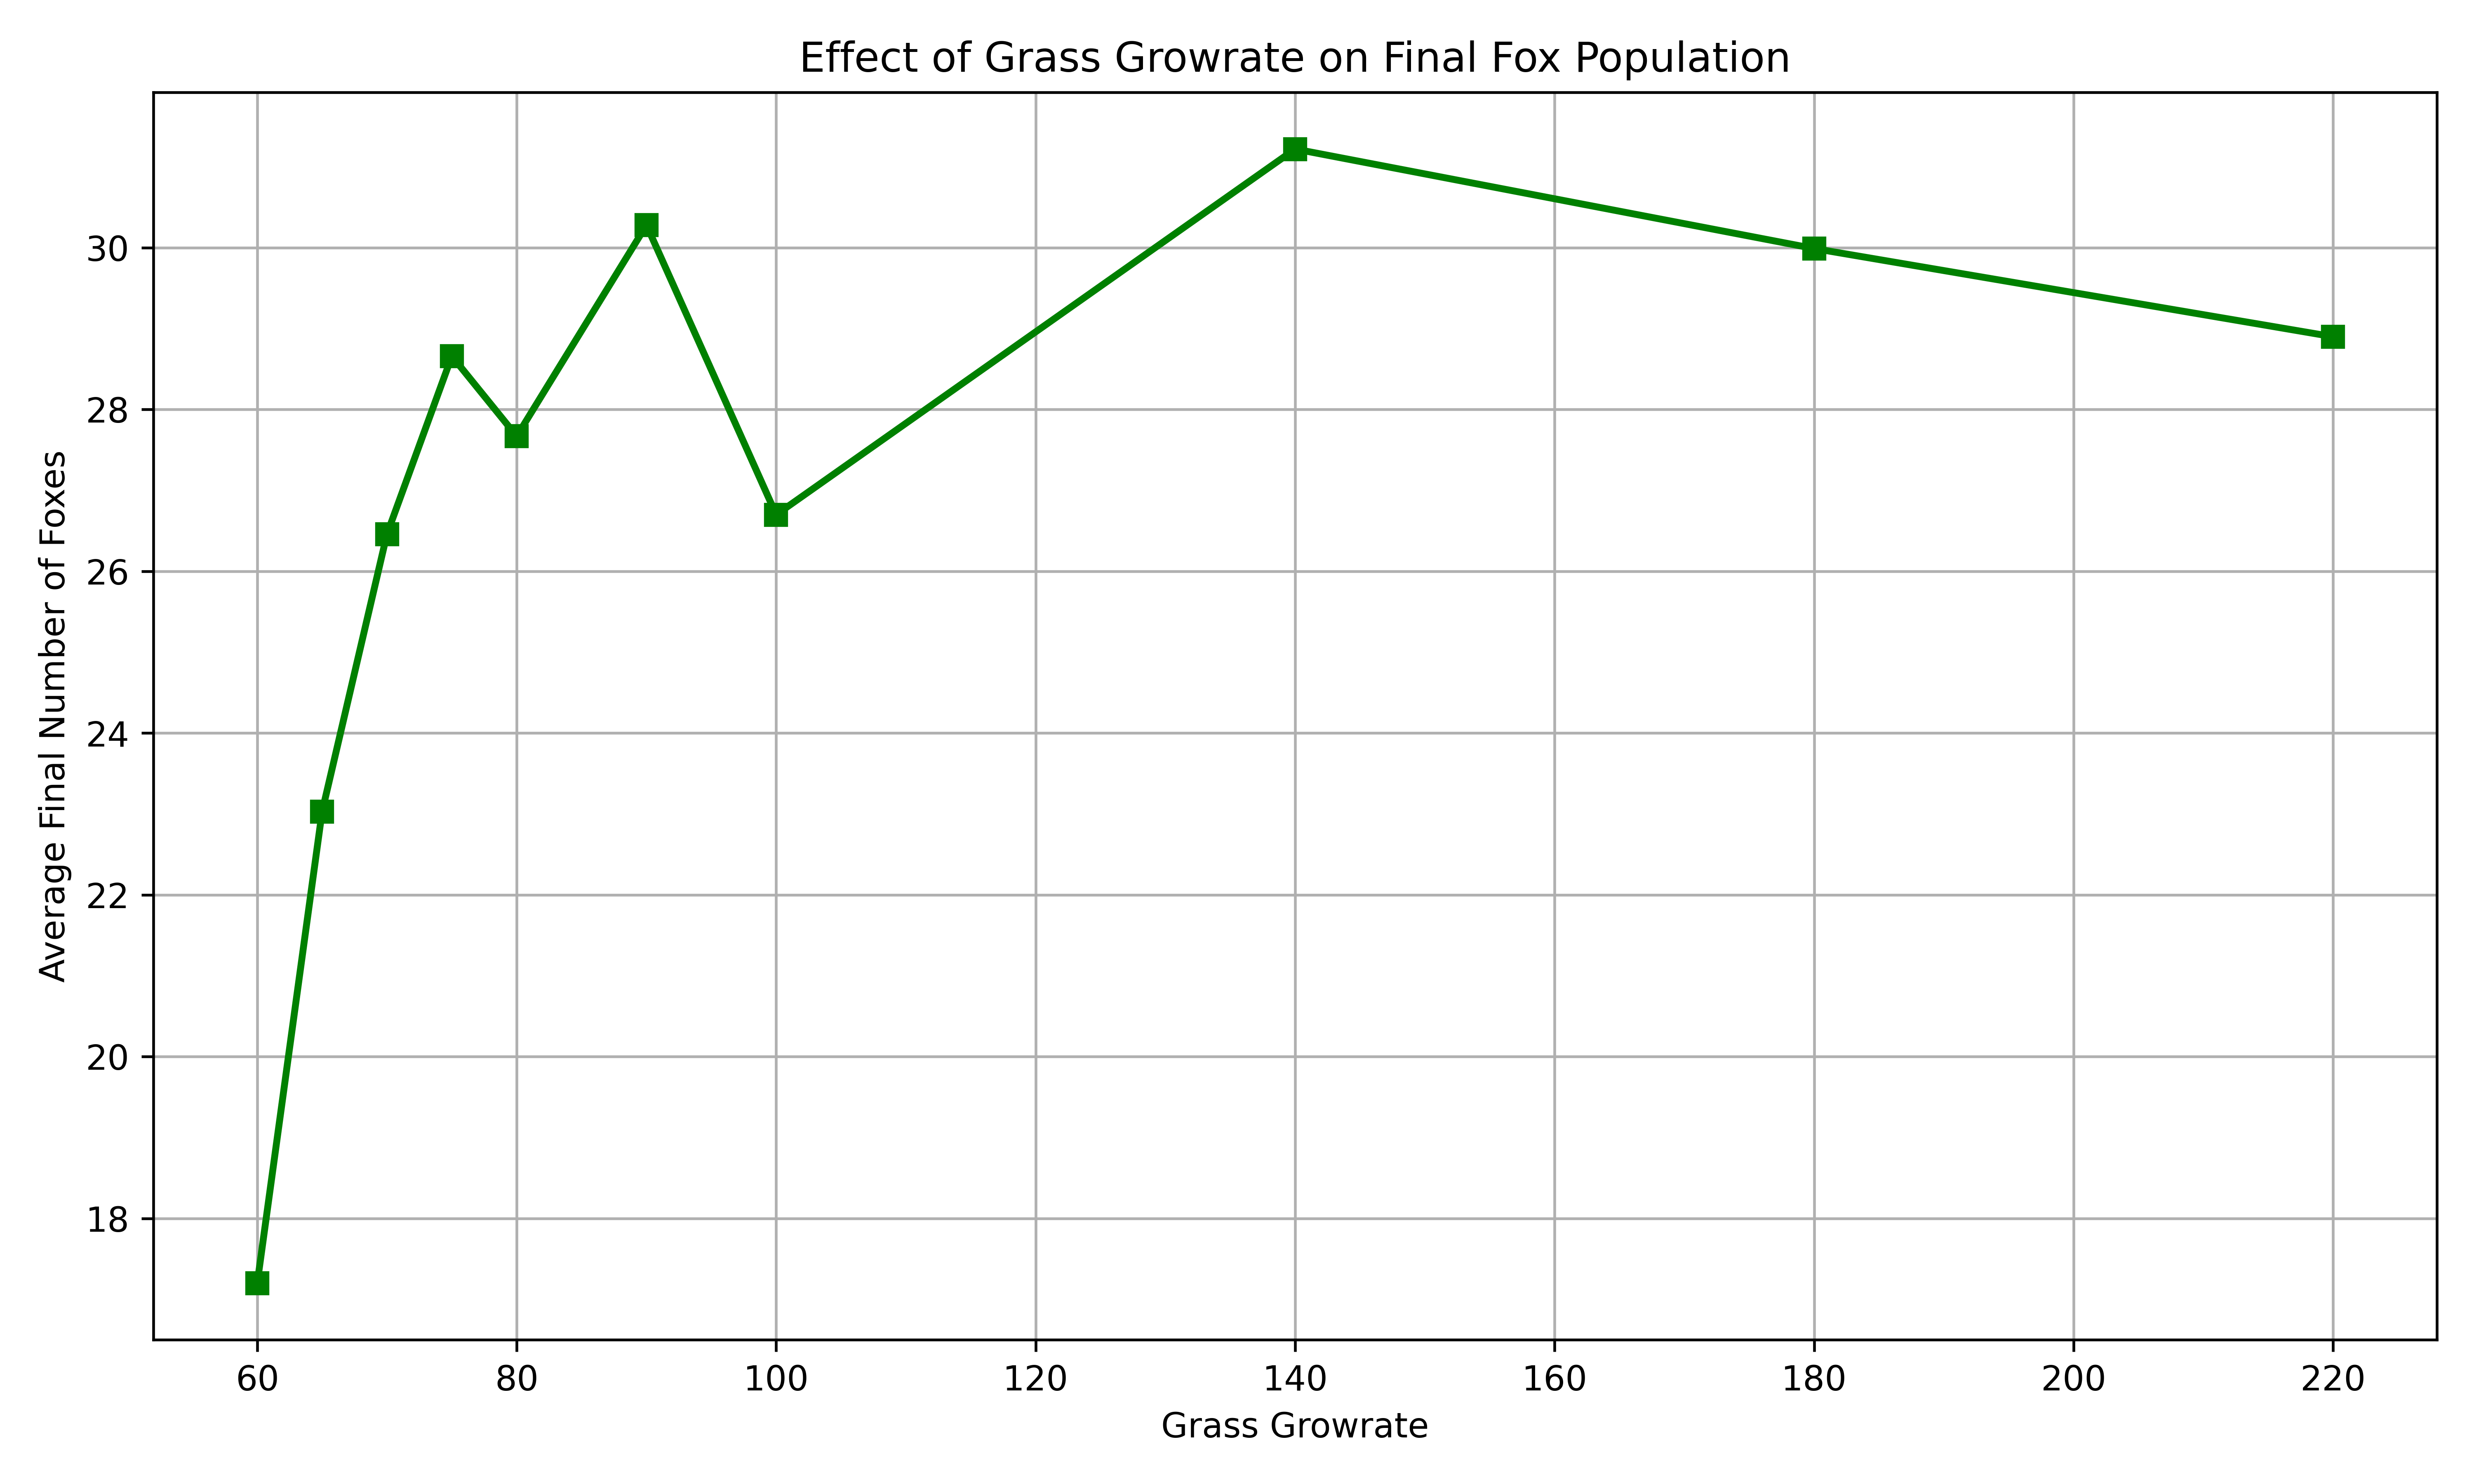
\includegraphics[width=0.9\linewidth]{images/avg_final_foxes_vs_growrate_100.png}
  \caption{
    Average final foxes vs growrate, recorded across 100 independent simulation runs of the Agent-Based Model (ABM), with each run 1000 iterations. For more information see Table ~\ref{tab:simulation_stats_2.1}.
}
  \label{fig:avg_final_foxes_vs_growrate_100_2.1}
\end{figure}



\begin{figure}[!ht]
  \centering
  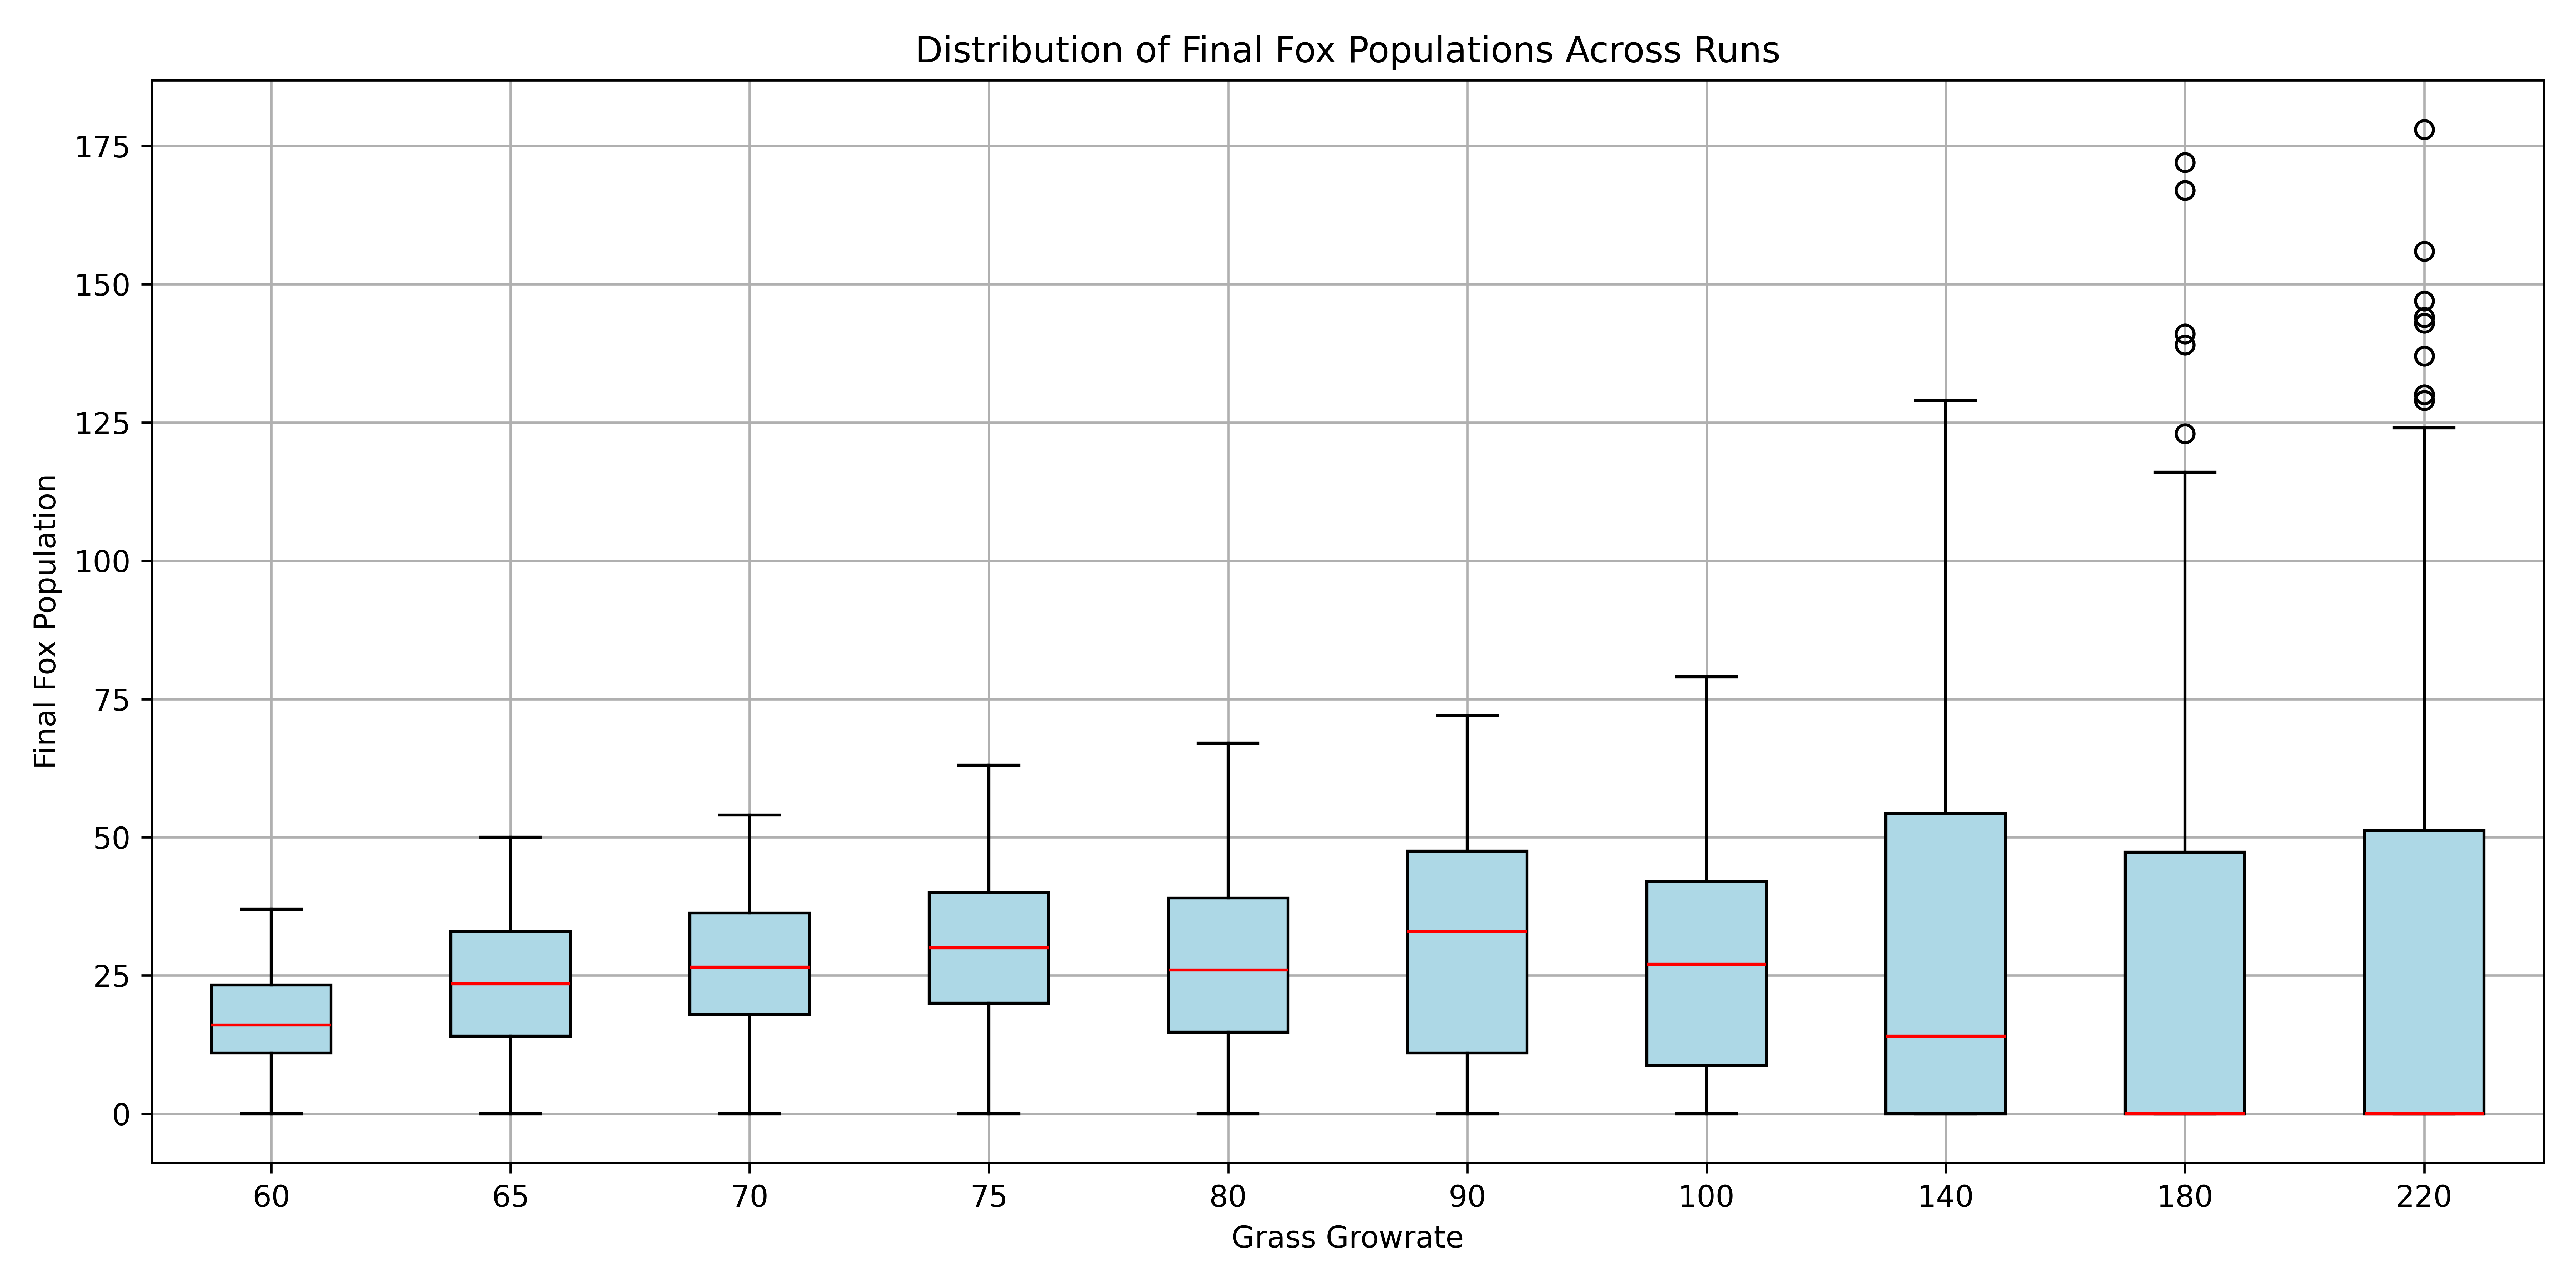
\includegraphics[width=0.9\linewidth]{images/boxplot_final_foxes_by_growrate_100.png}
  \caption{
    Final foxes by growrate, recorded across 100 independent simulation runs of the Agent-Based Model (ABM), with each run 1000 iterations. For more information see Table ~\ref{tab:simulation_stats_2.1}.
}
  \label{fig:boxplot_final_foxes_by_growrate_100_2.1}
\end{figure}

% \begin{figure}[!ht]
%   \centering
%   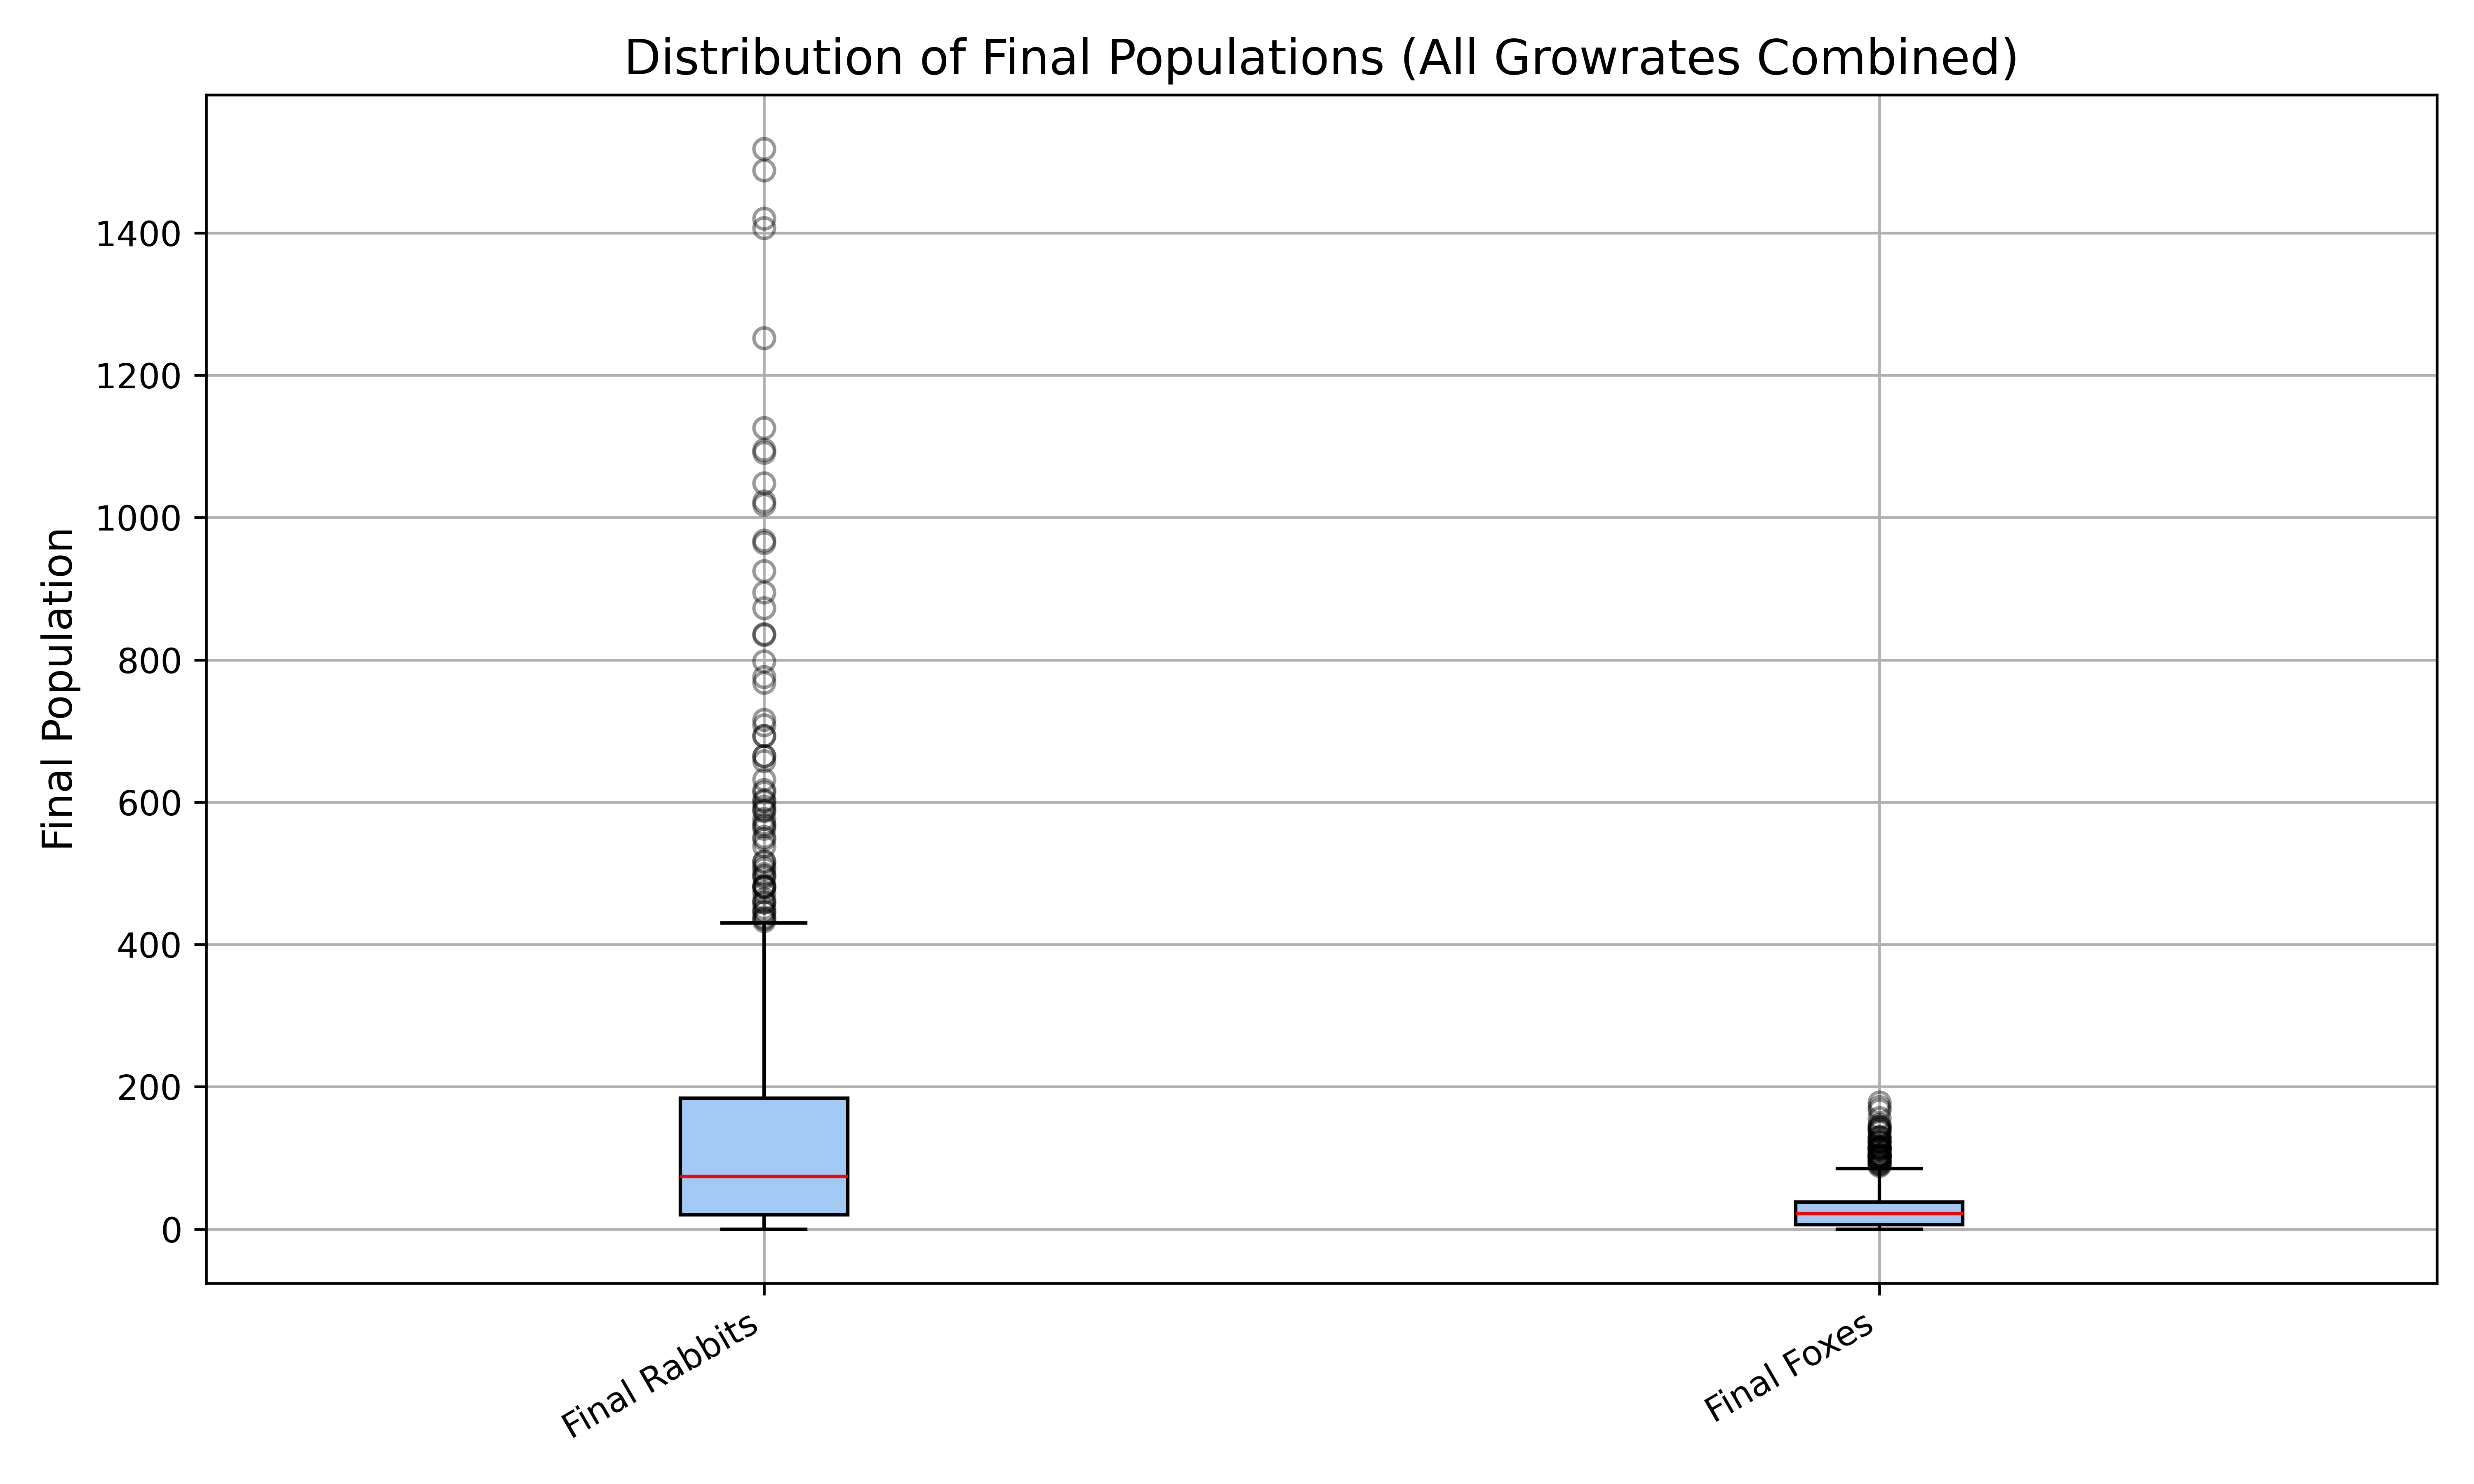
\includegraphics[width=0.9\linewidth]{images/boxplot_final_metrics_all_growrates_100.png}
%   \caption{
%     Descriptive statistics of key ecological variables recorded across 100 independent simulation runs of the Agent-Based Model (ABM), with each run 1000 iterations. For more information see Table ~\ref{tab:simulation_stats_2.1}.
% }
%   \label{fig:boxplot_final_metrics_all_growrates_100_2.1}
% \end{figure}




\begin{figure}[!ht]
  \centering
  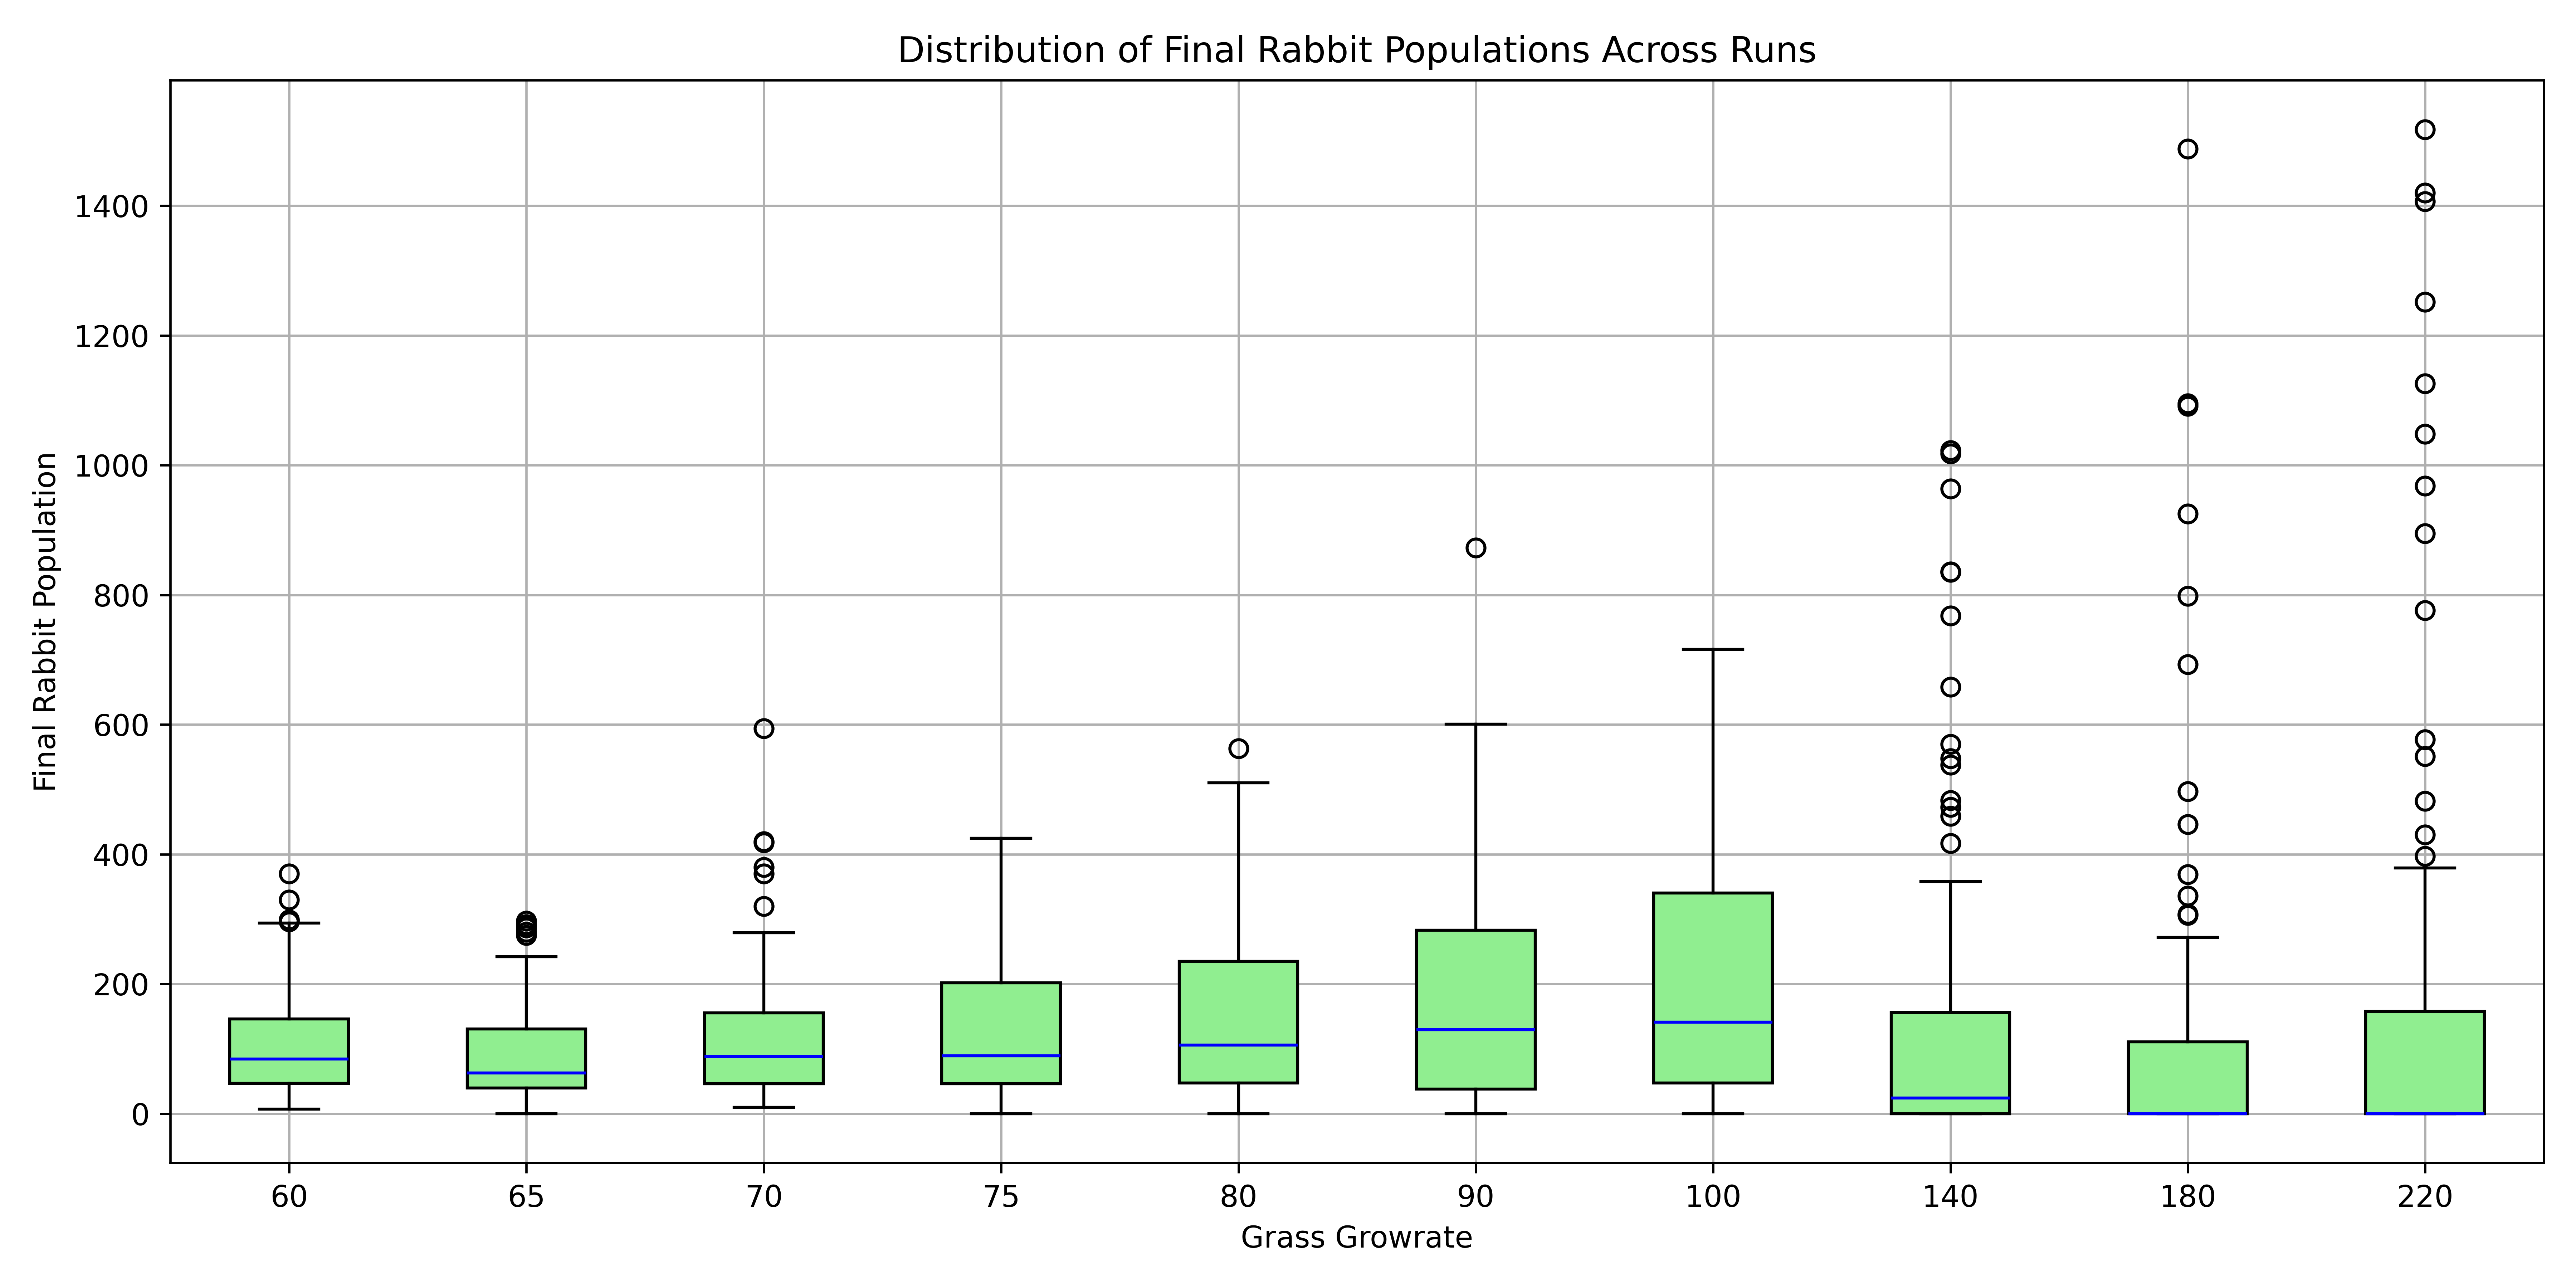
\includegraphics[width=0.9\linewidth]{images/boxplot_final_rabbits_by_growrate_100.png}
  \caption{
    Final rabbits by growrate, recorded across 100 independent simulation runs of the Agent-Based Model (ABM), with each run 1000 iterations. For more information see Table ~\ref{tab:simulation_stats_2.1}.
}
  \label{fig:boxplot_final_rabbits_by_growrate_100_2.1}
\end{figure}


\begin{figure}[!ht]
  \centering
  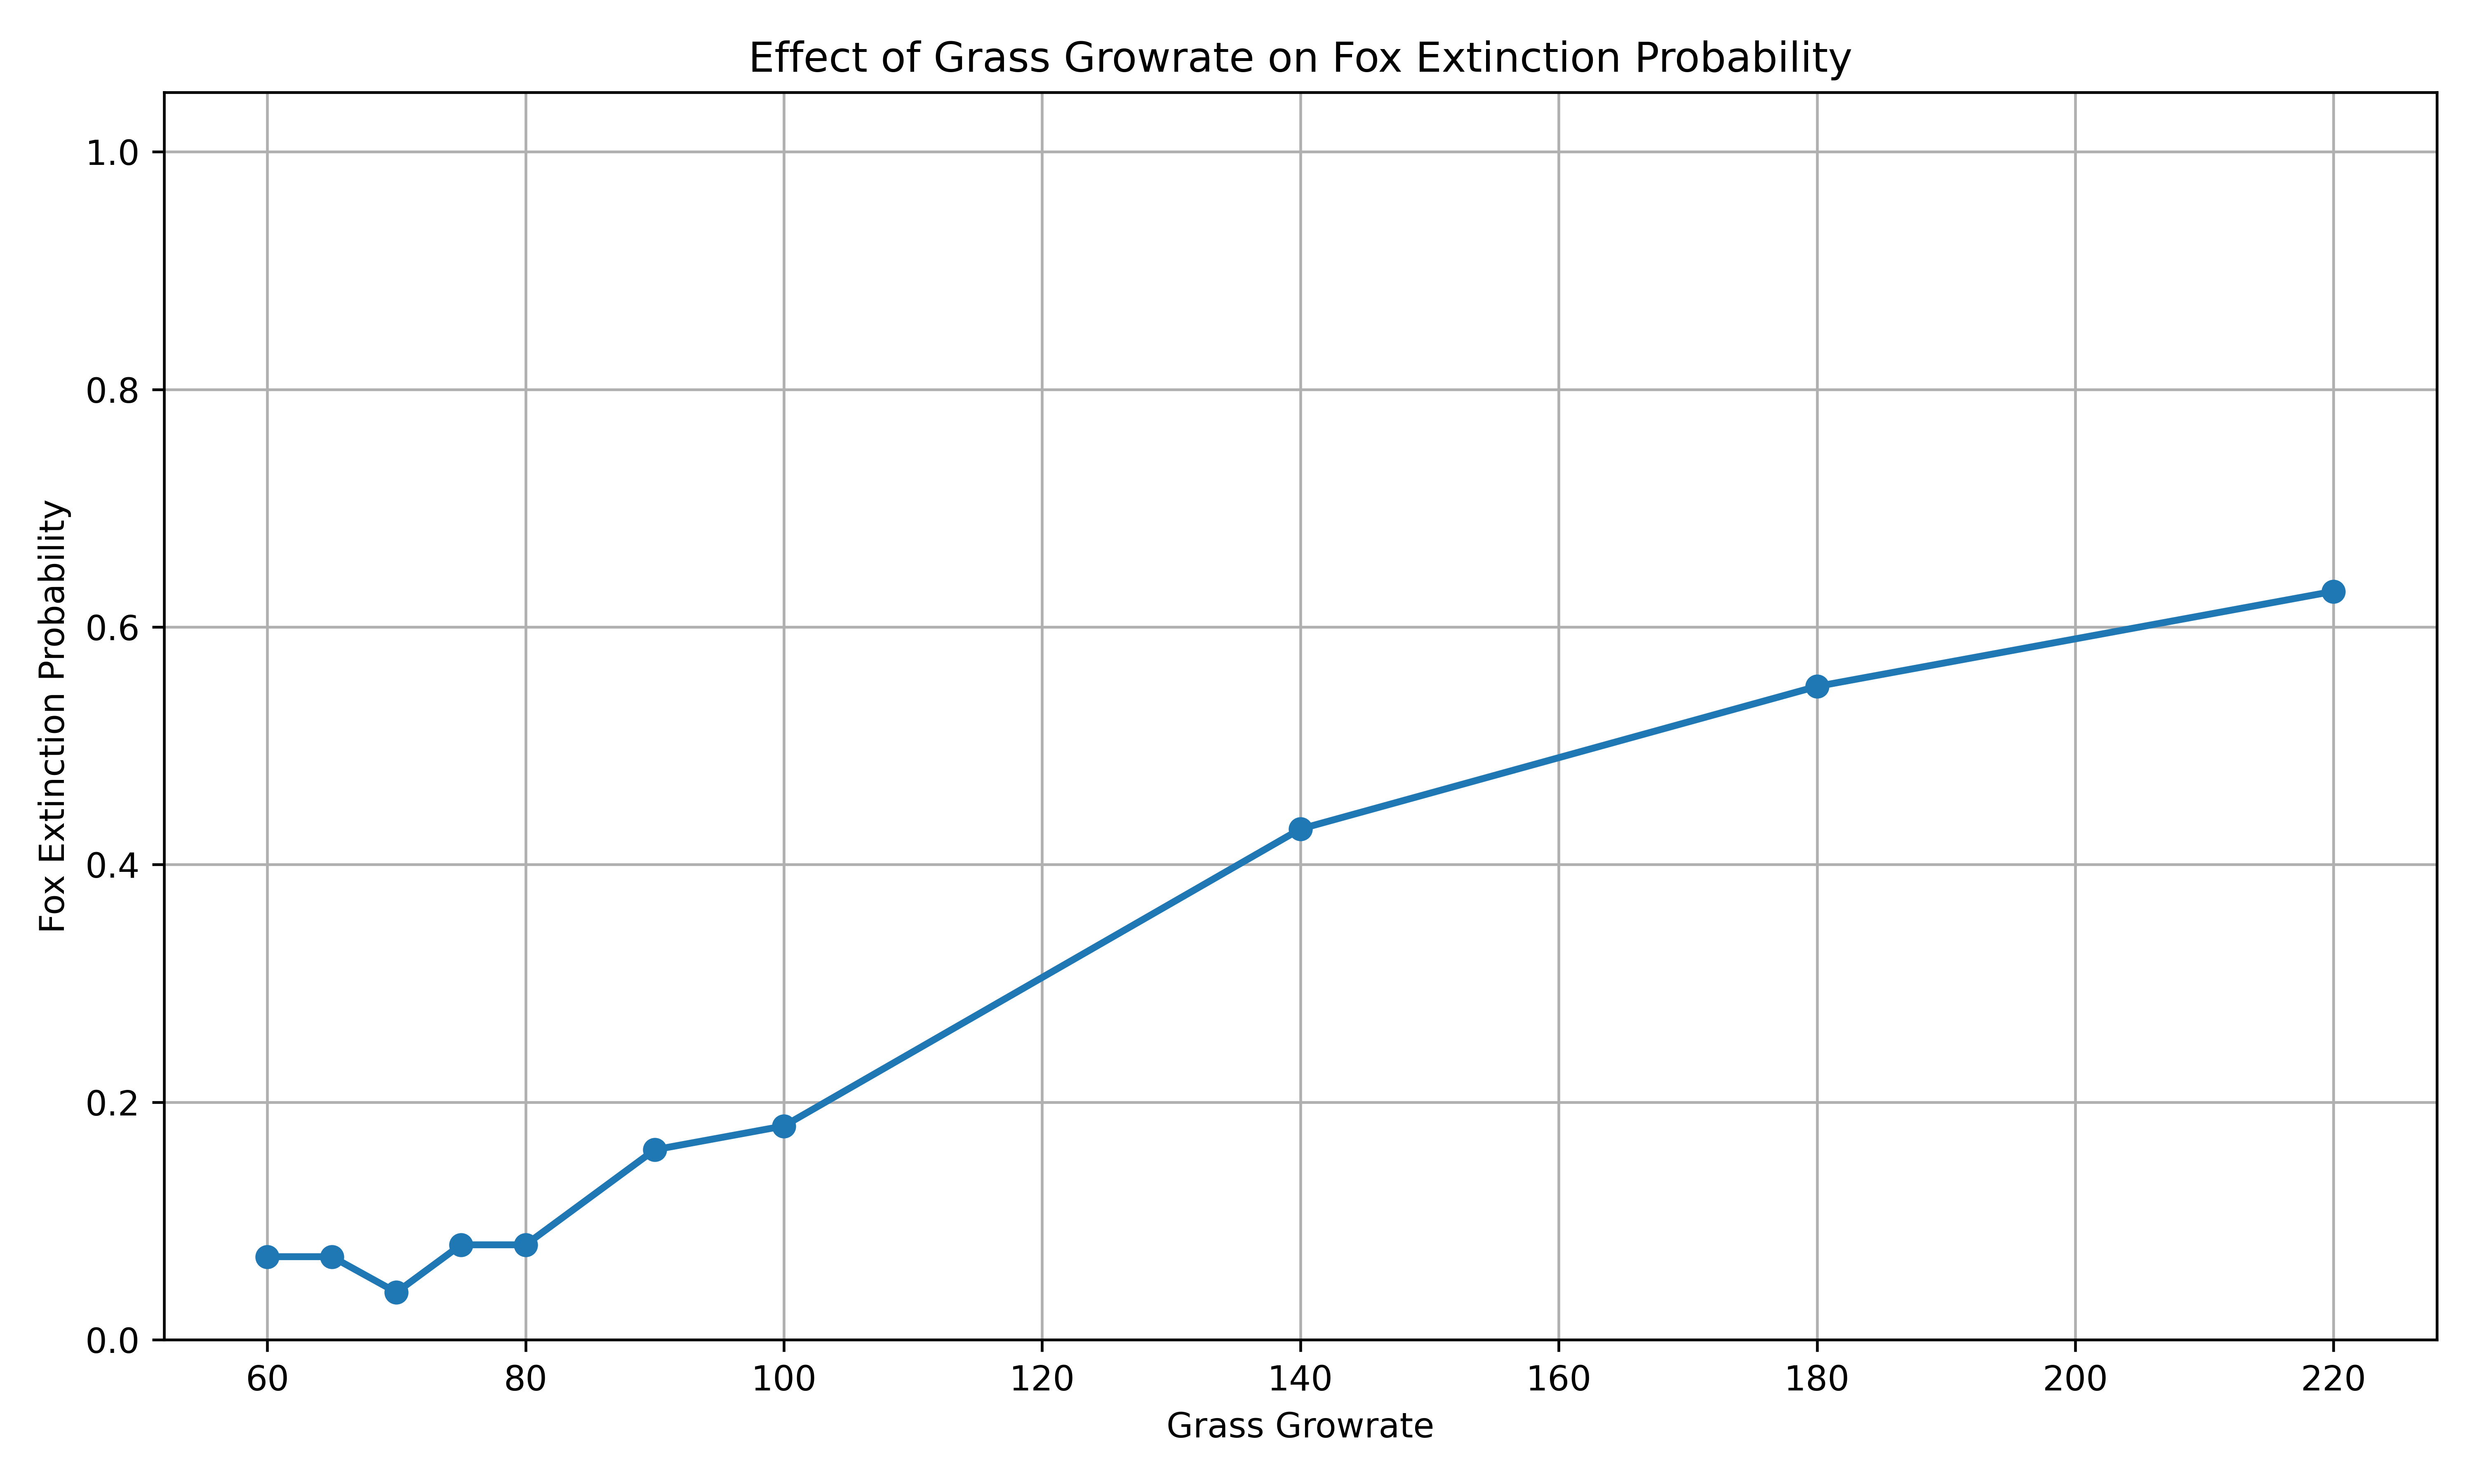
\includegraphics[width=0.9\linewidth]{images/fox_extinction_vs_growrate_100.png}
  \caption{
    Fox extinction vs growrate, recorded across 100 independent simulation runs of the Agent-Based Model (ABM), with each run 1000 iterations. For more information see Table ~\ref{tab:simulation_stats_2.1}.
}
  \label{fig:fox_extinction_vs_growrate_100_2.1}
\end{figure}